% -----------------------------------------------------------------
% Vorlage fuer Ausarbeitungen von
% Bachelor- und Masterarbeiten am ISS
% 
% Template for written reports or master theses at the ISS
% 
% For use with compilers pdflatex or latex->dvi2ps->ps2pdf.
%
% -----------------------------------------------------------------
% README, STUDENT USERS:
% We highly appreciate students using this template _AS IS_,period. 
% The document provides adjustable document preferences, 
% student information settings and typography definitions. Look for
% code delimited by *** ***
%
% The short explanation: it's the ISS common standard and 
% 	it's battle tested.
% The long explanation: 
%	We do not want you to go through the document and tweak the 
%	package options, layout parameters and line skips here and 
%	there and waste hours. We are providing this template such 
%	that you can fully concentrate on filling in the much more 
%	important _contents_ of your thesis.
%
% If you have serious needs on extra packages or design 
% modifications, talk to your supervisor _before_ modifying 
% the template.
% Similarly, we're happy if you give your supervisor a hint on any 
% errors in this template.
%
% -----------------------------------------------------------------
% History:
% Jan Scheuing,   04.03.2002
% Markus Buehren, 20.12.2004
% last changes:   10.01.2008 (removed unused packages), 
% 		07.08.2009 (added IEEEtran_LSS.bst file)
% 		02.05.2011 removed matriculation number from cover page
% Martin Kreissig, 25.01.2012: all eps/ps parts removed for 
% 				pdflatex to work properly
% Peter Hermannstaedter, 14.08.2012: fusion of versions for 
% 		latex/dvi/ps/pdf and pdflatex, additional comments,
% 		unification of document flags and student options
% Florian Liebgott, 12.03.2015: bug fixes, removal of obsolete options,
%		switch to UTF-8
% Florian Liebgott, 20.05.2015: fixed encoding problem on title page
% Florian Liebgott, 24.01.2017: changed deprecated font commands (like
%		\sl) to up-to-date commands to be compatible with
%		current TeX distributions.
% Felix Wiewel, 30.08.2021: Replace obsolete scrpage2 with scrlayer-scrpage
%
% -----------------------------------------------------------------
% If you experience any errors caused by this template, please
% contact Florian Liebgott (florian.liebgott@iss.uni-stuttgart.de)
% or your supervisor, so we can fix the errors.
% -----------------------------------------------------------------


\documentclass[12pt,DIV14,BCOR12mm,a4paper,footinclude=false,headinclude,parskip=half-,twoside,openright,cleardoublepage=empty,toc=index,bibliography=totoc,listof=totoc]{scrreprt}
% encoding needs to be defined here, otherwise umlauts on the titelpage won't work.
\usepackage[utf8]{inputenc}
%
%
%
% *****************************************************************
% -------------------> document preferences here <-----------------
% *****************************************************************
% Uncomment the settings you like and comment the settings you don't
% like.

% Language: 
% affects generic titles, Figure term, titlepage and bibliography
% (Note:if you switch the language, compile tex and bib >2 times)
\def \doclang{english} 	% For theses/reports in English
%\def \doclang{german} 		% For theses/reports in German

% Hyperref links in the document:
\def \colortype{color} % links with colored text
%\def \colortype{bw} 	% plain links, standard text color (e.g. for print)
%\def \colortype{boxed} % links with colored boxes
% *****************************************************************
%
%
%
% *****************************************************************
% --------------> put student information here <------------------
% *****************************************************************
% Please fill in all items denoted by "to be defined (TBD)"
\def \deworktitle{}        % German title/translation
\def \enworktitle{Avoiding Shortcut-Learning Through Mutual Information Minimization for Datasets with Multiple Confounding Variables}        % English title/translation
\def \tutor{Louisa Fay}
\def \student{Gautham Mohan}
\def \worksubject{Forschungsarbeit S1455}  % type and number (S/Dxxxx) of your thesis
\def \startdate{17/10/2023}
\def \submission{16/04/2024}
\def \signagedate{16/04/2024}   % Date of signature of declaration on last page
\def \keywords{Causality, deep learning}
\def \abstract{\textbf{Abstract}}

% *****************************************************************
%


\usepackage{amsmath}
\usepackage{amsfonts}
\usepackage{ifthen}
\ifthenelse{\equal{\doclang}{german}}{
	\usepackage[ngerman]{babel} %german version
	\def \maintitle{\deworktitle}
	\def \translatedtitle{\enworktitle}
	% set , to decimal and . to thousands separator, if German language is used
	\DeclareMathSymbol{,}{\mathord}{letters}{"3B}
	\DeclareMathSymbol{.}{\mathpunct}{letters}{"3A}
	}{
	%english version
	\def \maintitle{\enworktitle}
	\def \translatedtitle{\deworktitle}
	}
\usepackage{txfonts} % Times-Fonts
\usepackage[T1]{fontenc}
\usepackage{color}
\usepackage[headsepline]{scrlayer-scrpage} % Headings

\usepackage{svg}
\usepackage{graphicx}
\usepackage[format=hang]{caption}       % for hanging captions
\usepackage{subfig}                     % for subfigures
\usepackage{wrapfig}                    % for figures floating in text, alternatively you can use >>floatflt<<
\usepackage{booktabs}                   % nice looking tables (for tables with ONLY horizontal lines)
\usepackage{float}
\usepackage{algorithm}
\usepackage{algpseudocode}
\usepackage{diagbox}
\usepackage{tabularx}
%%%%% Tikz / PGF - drawing beautiful graphics and plots in Latex
% \usepackage{tikz}
% \usetikzlibrary{plotmarks}              % larger choice of plot marks
% \usetikzlibrary{arrows}                 % larger choice of arrow heads
% % ... insert other libraries you need
% \usepackage{pgfplots}
% % set , to decimal and . to thousands separator for plots, if German language is used
% \ifthenelse{\equal{\doclang}{german}}{
% \pgfkeys{/pgf/number format/set decimal separator={,}}
% \pgfkeys{/pgf/number format/set thousands separator={.}}
% }{}
%%%%%%

\ifthenelse{\equal{\colortype}{color}}{
	% colored text version:
	\usepackage[colorlinks,linkcolor=blue]{hyperref}
	\newcommand{\bugfix}{\color{white}{\texttt{\symbol{'004}}}} % Bug-Fix Umlaute in Verbatim
}{
	\ifthenelse{\equal{\colortype}{boxed}}{
		% colored box version:
		\usepackage{hyperref}
		\newcommand{\bugfix}{\color{white}{\texttt{\symbol{'004}}}} % Bug-Fix Umlaute in Verbatim
	}{
		% monochrome version:
		\usepackage[hidelinks]{hyperref}
		\newcommand{\bugfix}{\color{white}{\texttt{\symbol{'004}}}} % Bug-Fix Umlaute in Verbatim
	}
}

% Layout and Headings
\pagestyle{scrheadings}
\automark{chapter}
\clearscrheadfoot
\lehead[]{\pagemark~~\headmark}
\rohead[]{\headmark~~\pagemark}
\renewcommand{\chaptermark}[1]{\markboth {\normalfont\slshape \hspace{8mm}#1}{}}
\renewcommand{\sectionmark}[1]{\markright{\normalfont\slshape \thesection~#1\hspace{8mm}}}
\addtolength{\textheight}{15mm}
\parindent0ex
\setlength{\parskip}{5pt plus 2pt minus 1pt}
\renewcommand*{\pnumfont}{\normalfont\slshape} % Seitenzahl geneigt
\renewcommand*{\sectfont}{\bfseries} % Kapitelueberschrift nicht Helvetica

% Settings for PDF document
\pdfstringdef \studentPDF {\student} 
\pdfstringdef \worktitlePDF {\maintitle}
\pdfstringdef \worksubjectPDF {\worksubject}
\hypersetup{pdfauthor=\studentPDF, 
            pdftitle=\worktitlePDF,
            pdfsubject=\worksubjectPDF}

% Title page
\titlehead{
	\includegraphics[width=20mm]{university-logo}
	\hspace{6mm}
	\ifthenelse{\equal{\doclang}{german}}{
		\begin{minipage}[b]{.6\textwidth}
		{\Large Universit\"at Stuttgart } \\
		Institut f\"ur Signalverarbeitung und Systemtheorie\\
		Professor Dr.-Ing. B. Yang \vspace{0pt}
		\end{minipage}
	}{
		\begin{minipage}[b]{.6\textwidth}
		{\Large University of Stuttgart } \\
		Institute for Signal Processing and System Theory\\
		Professor Dr.-Ing. B. Yang \vspace{0pt}
		\end{minipage}
	}
	\hspace{1mm}
	\includegraphics[width=28mm]{isslogocolor}
}
\subject{\worksubject\vspace*{-5mm}} % Art und Nummer der Arbeit
\title{\maintitle}%\\ \Large{\subtitle}}
\subtitle{\translatedtitle}
\author{
\large
  \ifthenelse{\equal{\doclang}{german}}{
  \begin{tabular}{rp{7cm}}
    \Large 
    Autor:      & \Large \student \vspace*{2mm}\\
    Ausgabe:    & \startdate \\
    Abgabe:     & \submission \vspace*{3mm}\\
    Betreuer:   & \tutor \vspace*{2mm}\\
    Stichworte: & \keywords
  \end{tabular}
  }{
  \begin{tabular}{rp{7cm}}
    \Large 
    Author:             & \Large \student \vspace*{2mm}\\
    Date of work begin: & \startdate \\
    Date of submission: & \submission \vspace*{3mm}\\
    Supervisor:         & \tutor \vspace*{2mm}\\
    Keywords:           & \keywords 
  \end{tabular}
  }
  \bugfix
}

\date{}
\publishers{\normalsize
  \begin{minipage}[t]{.9\textwidth}
    \abstract
        \hspace{0.02\linewidth}
        Deep learning methodologies rely on the ability to leverage relationships between features within datasets to extract meaningful representations. However, confounding variables can introduce spurious or meaningless correlations into the dataset, leading to biases in deep learning models. The mutual information minimization model successfully learns causal relationships from datasets with a single confounding variable. This thesis proposes an extension of the concept for datasets with multiple confounding variables. A detailed study of the mutual information neural estimation and an exploration of the causal structure of datasets with multiple confounding variables have been done for this. The proposed model has been tested on two datasets - a benchmark Morpho-MNIST dataset and a medical CheXpert dataset. The experiments performed validate the success of the model in learning true causal relationships from datasets with multiple confounding variables.
  \end{minipage}
}

\numberwithin{equation}{chapter} 
\sloppy 

%
%
%
% *****************************************************************
% --------------> put typography definitions here <----------------
% *****************************************************************
% colors
\definecolor{darkblue}{rgb}{0,0,0.4}

% declarations
\newcommand{\matlab}{\textsc{Matlab}\raisebox{1ex}{\tiny{\textregistered}} }
% Integers, natural, real and complex numbers
\newcommand{\Z}{\mathbb{Z}}
\newcommand{\N}{\mathbb{N}}
\newcommand{\R}{\mathbb{R}}
\newcommand{\C}{\mathbb{C}}
% expectation operator
\newcommand{\E}{\operatorname{E}}
% imaginary unit
\newcommand{\im}{\operatorname{j}}
% Euler's number with exponent as parameter, e.g. \e{\im\omega}
\newcommand{\e}[1]{\operatorname{e}^{\,#1}}
% short command for \operatorname{}
\newcommand{\op}[1]{\operatorname{#1}}

% unknown hyphenation rules
\hyphenation{Im-puls-ant-wort Im-puls-ant-wort-ko-ef-fi-zien-ten
Pro-gramm-aus-schnitt Mi-kro-fon-sig-nal}
% *****************************************************************
%
\begin{document}

% title and table of contents
\pagenumbering{alph}
\maketitle
\cleardoublepage
\pagenumbering{roman} % roman numbering for table of contents
\tableofcontents
\cleardoublepage
\setcounter{page}{1}
\pagenumbering{arabic} % arabic numbering for rest of document

% *****************************************************************
% -------------------> start writing here <------------------------

\chapter{Introduction}
The development of convolutional neural networks (CNNs) has catalysed a shift in computer vision, moving away from expert systems towards deep learning \cite{litjens_2017_a}. Although gradual, the medical imaging community has also undergone this change, employing deep learning for various applications such as segmentation, classification, and detection across a range of data types including MRI, microscopy, CT scans, and X-rays. Notably, leading participants in various challenges in computer-aided diagnostics (CAD), such as those on Kaggle and in DREAM challenges, consistently rely on deep learning techniques \cite{tsuneki_2022_deep}.

Learning algorithm often assume that features in training and test dataset are independent and identically distributed \cite{788640}.But this assumption does not hold in real-world, particularly in medical datasets. Distribution of features such as the sex and age of patients, as well as the hospital environment maybe skewed \cite{larrazabal_2020_gender} \cite{sanchez_2022_causal} \cite{dazrodrguez_2023_gender}. Such deviations from the ideal distribution can lead to the emergence of spurious non-predictive correlations\cite{lynch2023spawrious} \cite{DBLP:journals/corr/abs-2004-07780}.

Deep learning, which relies on learning associations between variables in the data, encounters challenges in distinguishing between causal relationships and mere spurious correlations \cite{sanchez_2022_causal} \cite{DBLP:journals/corr/abs-2004-07780}. While causal relationships are invariant to distribution shifts, spurious correlations are often tied to the distribution and can mislead the models to wrong results when the distribution changes, such as shifts in demography or hospital environments from which the data is collected \cite{DBLP:journals/corr/abs-1807-04975} \cite{DBLP:journals/corr/abs-1911-08731} \cite{sanchez_2022_causal}. These distribution shifts can have significant implications for the reliability and generalizability of predictive models.

The primary feature of a model that learns the true causal relationships in data is counterfactual invariance, i.e. the model should be able to predict the correct output label for a given input even if the spuriously correlated variable in the input changes \cite{DBLP:journals/corr/abs-2106-00545}. The process of bringing such invariance to the deep learning model requires an understanding of the causal structure of the original training data. To bring forth counterfactual invariance it is important to determine the degree of spurious correlation between two variables. Mutual information (MI) can be used as a measure for this purpose \cite{10162210}. A mutual information neural estimation (MINE) technique which relies on the Donsker-Varadhan representation of Kullback-Leibler (KL) divergence has been proposed by Belghazi et al.  \cite{DBLP:journals/corr/abs-1801-04062}.

Fay et. al. \cite{10162210} proposed a novel mutual information minimization model (MIMM) for datasets with a single spurious correlation variable. The framework requires a feature encoder combined with a MINE model to estimate MI and use it as a regularisation term in the loss function for classification tasks. This thesis is an extension of the concept for datasets with multiple spurious correlation variables.

\chapter{Literature Review}
The literature review was conducted to explore the basic foundations of causal inference and counterfactual invariance. MINE was studied as a method to quantify spurious correlation between variables, while also emphasizing essential considerations crucial for its application. Furthermore, a comprehensive examination of MIMM, as introduced by Fay et al., is provided, along with its intricate training process. The insights gained from this review are presented below in subsequent sections.

\section{Causal Background}
The basics to understanding causality is to understand that the existence of a correlation between two variables does not mean that one variable causes the other\cite{peters_2017_elements}\cite{ward_2012_spurious}. The idea behind this statement is that correlation is not a necessary or sufficient condition for causal relationships. Such correlations which has a tendency to imply a causal relationship between correlated event but actually does not mean anything of the same nature are called spurious correlations. 

Reichenbach's common cause principle suggests a mechanism by which spurious correlations can arise \cite{peters_2017_elements}. The statement suggests that given two variables \textit{Z} and \textit{Y} are statistically dependent i.e. $Z \not\perp\!\!\!\perp Y$,then there exists a third variable \textit{U} causally influencing both of them. In such cases, the \textit{Z} and \textit{Y} are independent of each other given we know the confounding variable \textit{U}, i.e. $Z\perp\!\!\!\perp Y\mid U$.

This is illustrated in \ref{fig:confounding} through an example, \textit{Z}="type of scanner" and \textit{Y}="type of neurological disease" and \textit{U}="Doctor" \cite{10162210}. Now assume that "Doctor A" is a specialist in Alzheimer's disease (AD) and works mostly with "Scanner A" and "Doctor B" attends mostly to general neurological disorders while using "Scanner B" for his procedures. This results in a data-generating process which shows a spurious correlation between AD and "Scanner A". However, this correlation is not causal; it is solely influenced by the doctor, i.e. \textit{U} treating the patients, i.e. we can independently determine the "type of scanner" and "type of neurological disease" from the knowledge of which "Doctor" is treating the patient.

\begin{figure}[H]
    \centering
    \includesvg[height=5cm]{figures/confounding} 
    \caption{Spurious correlation through confounding. The confounding variable is marked in red. The arrow marks the direction of causation and the spurious correlation is shown through the red dotted line.}
    \label{fig:confounding}
\end{figure}

The other common mechanism for spurious correlation which is often discussed in the medical domain in selection bias. This occurs when two independent variables \textit{Y} and \textit{Z} jointly cause an observation \textit{S} \cite{Pearl09}. Here although the \textit{Y} and \textit{Z} are marginally independent, when conditioned on \textit{S} they become dependent, i.e. $Z\not\perp\!\!\!\perp Y\mid S$. 

The selection bias is illustrated in \ref{fig:selection} through an example \cite{Pearl09}. Suppose a particular graduate school admits students either on the criteria that they have good grades or on the criteria they are exceptionally musically talented, then the grades and musical talent across the population of students admitted to the school will appear to be negatively correlated. Here, although the general population shows no particular correlation between musical talent and grades, if we select a single student admitted to the school and if the student has low grades then the student will obviously need to have higher musical talent to be admitted to the school.

\begin{figure}[H]
    \centering
    \includesvg[height=3.5cm]{figures/selection} 
    \caption{Spurious correlation through selection. The selection variable is marked in red. The arrow marks the direction of causation and the spurious correlation is shown through the red dotted line.}
    \label{fig:selection}
\end{figure}

Machine learning is essentially learning associations between input samples \textit{X} and their labels \textit{Y}, this is done in the training process by adjusting the parameters of a model \textit{f} to map \textit{X} to \textit{Y} \cite{sanchez_2022_causal} \cite{DBLP:journals/corr/abs-2106-00545}.This mapping from $X$ to $Y$ is said to be in the causal direction if $X$ is the cause of $Y$, an example would be humidity, temperature and wind speed ($X$) being used to predict the chance for rain ($Y$). The same mapping is said to be in the anti-causal direction if $Y$ is the cause for $X$, an example can be drawn from the MNIST dataset where the idea of the number "4" that is the label "4" ($Y$) is the cause for the shape of the number in its image input ($X$) \cite{10162210}.   

The concepts described above can be well summarized using the example of mophoMNIST image classification as provided by Fay et. al. \cite{10162210} illustrated in \ref{fig:anti-causal_confounding}. In this example a writer "A" uses thick nib pens and writes mostly high-valued numbers like "9" while another writer "B" uses thin nib pens to write mostly low-valued numbers like "2". This end up in a process that creates spurious correlation between the numbers ranging from 0-4 ("low") and thin profile, and the numbers in the range 5-9 ("high") and thick profile, the profile being the spurious correlation variable $Z$ and the writer $U$ being the confounding variable. The label $Y$ is the primary task to be predicted by the model $f$ from the input image $X$, this is indicated by green thick arrow. The value taken by label, i.e. "high" or "low" and the profile chosen, i.e. "thick" or "thin" determines the kind of image that we get, hence the direction of causation along the black arrows as indicated. 

\begin{figure}[htbp]
    \centering
    \includegraphics[height=5cm]{thesis/figures/anti-causal_confounding_new.png} 
    \caption{Predictions in anti-causal directions in a confounded Morpho-MNIST dataset.}
    \label{fig:anti-causal_confounding}
\end{figure}

\section{Counterfactual Invariance}

In Figure \ref{fig:counterfactuals} we see that $X$ is causally influenced by $Y$ and $Z$ \cite{10162210}. This means that in the image $X$ of the number of "4", there is a representation of the label $Y="4"$ as the shape of the number and the thickness $Z$ of the number $Z$. Now, if we fix the value of $Y="4"$ and then vary the value of $Z$ between "thick" and "thin" we get a counterfactual pair of $X$. We can formalise such counterfactuals as $X(y,z)$ and $X(y,z')$, in the example $z$ and $z'$ correspond to "thick" and "thin" and $y$ is fixed which is "4" here \cite{DBLP:journals/corr/abs-2106-00545}.

\begin{figure}[htbp]
    \centering
    \includegraphics[height=5cm]{figures/counterfactuals.png} 
    \caption{Counterfactuals generated by varying the thickness of lines pen used to write the number 4.}
    \label{fig:counterfactuals}
\end{figure}

A neural network is a function $f$ which takes $X$ as input to make a prediction about the label $Y$. The variable $Y$ here refers to the ground truth and the actual prediction is represented by $f(X)$. The predictions of such a model is said to be counterfactually invariant if it satisfies the following condition-

\begin{equation} \label{eq:counterfactual_invariance_1}
    f(X(y,z)) = f(X(y,z'))
\end{equation}

This means that the prediction $f(X)$ remains the same even if $Z$ changes ("independent of $Z$"), as long as the value of $Y=y$ remains fixed ("given $Y$"). Hence the above condition can be re-written as below-

\begin{equation} \label{eq:counterfactual_invariance_2}
    f(X) \perp\!\!\!\perp Z \mid Y 
\end{equation}

This implies that $f$ learns the representation of $Y$ embedded in $X$ and ignores the representatio of $Z$ in it. For the example in Figure \ref{fig:counterfactuals} this would mean that the neural network learns the shape of the number by ignoring the information about thickness embedded in the image. However, the neural network cannot learn representations of the label $Y$ from $X$ in isolation, this is because of the presence of confounding variables that create spurious correlation between $Y$ and $Z$, confusing the network into using $Z$ to predict $Y$ \cite{DBLP:journals/corr/abs-2109-05642} \cite{DBLP:journals/corr/abs-2106-00545}. 

In the example illustrated in Figure \ref{fig:anti-causal_confounding}, here all the samples that are "thick" are also "high" and all the samples that are "thin" are also "low". This information is embedded in the input image $X$ which could result in the model relying on the information that the image $X$ has a thick profile to predict that the number belongs to "high" class \cite{10162210}. Let there be an input $x=X(Y="small", Z="thick")$, this is an out-of-domain image since there is no image similar to the given $x$ present in the original training set. Since $f$ learned the spurious correlation between thickness and the label, it is probable that the model will now predict $x$ to belong to class "high" even though it actually does not belong to it \cite{DBLP:journals/corr/abs-2109-05642}. To avert this and enhance the model's out-of-domain generalization, we must sever the spuriously correlated connection between $X$ and $Z$ \cite{10162210}.

\section{Mutual Information Neural Estimation}\label{sec: 2.3}
The previous sections explain how spurious correlation between some features in the data and the label can reduce the ability of machine learning models to generalise well to the data. To prevent the occurrence of spurious correlation, it is necessary to able quantify it. 

While linear correlation measures can be used to gauge spurious correlation, it has the limitation that it only captures linear relationships. It merely indicates whether one variable increases or decreases as the other increases but often the relationships between features in a dataset is much more complex and a simple linear relationship might not be able to capture this. MI serves as a robust measure that can be utilized in this scenario. \cite{Li1990} \cite{10162210}.

MI is a measure based on shannon entropy as summarised by the expression \ref{eq:shannon_mi} \cite{DBLP:journals/corr/abs-1801-04062}. This can be interpreted as the information gained about $Y$ from the knowledge of $Z$, which also can be interpreted as the dependence of $Y$ on $Z$. 

\begin{equation}\label{eq:shannon_mi}
    I(Y;Z) = H(Y) - H(Y|Z)
\end{equation}

It can also be represented using KL divergence as \ref{eq:KL_MI} \cite{DBLP:journals/corr/abs-1801-04062}. The higher the divergence between the joint distribution and product of the marginal distributions of $X$ and $Z$ the higher the MI between them, this also corresponds to the independence criteria where $Y$ and $Z$ are independent if $\mathbb{P}_{YZ} = \mathbb{P}_Y \otimes \mathbb{P}_Z$.

\begin{equation}\label{eq:KL_MI}
    I(Y;Z) = D_{\text{KL}}(\mathbb{P}_{YZ} \| \mathbb{P}_Y \otimes
 \mathbb{P}_Z)
\end{equation}

The expression \ref{eq:KL_MI} cannot be used directly and a more tractable form of the equation is available through the Donsker-Varadhan representation of KL-divergence as given in expression \ref{eq:KL_DV} \cite{DBLP:journals/corr/abs-1801-04062}. Here we are taking supremum over all functions $T$ that maps from the sample space $\Omega$ to a real number $\mathbb{R}$.  

\begin{equation}\label{eq:KL_DV}
    D_{\text{KL}}(\mathbb{P}\|\mathbb{Q}) =  \sup_{T: \Omega \rightarrow \mathbb{R}} \left( \mathbb{E}_\mathbb{P}[T] - \log(\mathbb{E}_\mathbb{Q}[e^T]) \right)
\end{equation}

MINE uses a neural network to model $T$ and it now belongs to a class of functions $\mathcal{F}$, this network is called the statistics network. Since the range of functions that can be represented by the statistics network is limited, it now represents a tight lower bound for KL divergence. The expression \ref{eq:KL_DV} can now be adapted for KL divergence given in expression \ref{eq:KL_MI} with $T: Y \times Z \rightarrow \mathbb{R} $ parameterized by $\theta$ of the network \cite{DBLP:journals/corr/abs-1801-04062}.

\begin{equation}\label{eq:DV_MI}
    D_{\text{KL}}(\mathbb{P}_{YZ}\|\mathbb{P}_Y \otimes
 \mathbb{P}_Z) =  \sup_{\theta \in \Theta} \left( \mathbb{E}_{\mathbb{P}_{YZ}}[T_{\theta}(Y,Z)] - \log(\mathbb{E}_{\mathbb{P}_{Y} \otimes
 \mathbb{P}_Z}[e^{T_{\theta}(Y',Z')}]) \right)
\end{equation}

The samples from the independent distribution $(Y',Z') \sim \mathbb{P}_Y \otimes
 \mathbb{P}_Z$ can be produced by shuffling the samples from the joint distribution $(Y, Z) \sim \mathbb{P}_{YZ}$. In order to find the supremum the term in expression \ref{eq:DV_MI} is maximised using stochastic gradient descent (SGD). The gradient of \ref{eq:DV_MI} with respect to $\theta$ yields us expression \ref{eq:DV_MI_GRAD}, here $B$ represents a mini-batch \cite{DBLP:journals/corr/abs-1801-04062}. MINE is strongly consistent given that we have a sufficient batch size and a statistics network $T_{\theta}$ with sufficient representational power.

 \begin{equation}\label{eq:DV_MI_GRAD}
\widehat{G}_{B}=\mathbb{E}_{B}\left[\nabla_{\theta} T_{\theta}\right]-\frac{\mathbb{E}_{B}\left[\nabla_{\theta} T_{\theta} e^{T_{\theta}}\right]}{\mathbb{E}_{B}\left[e^{T_{\theta}}\right]},
\end{equation}

 \begin{equation}\label{eq:SGD_issue_mine}
\frac{\mathbb{E}_{B}\left[\nabla_{\theta} T_{\theta} e^{T_{\theta}}\right]}{\mathbb{E}_{B}\left[e^{T_{\theta}}\right]}\neq \frac{\nabla_{\theta} T_{\theta} e^{T_{\theta}}}{e^{T_{\theta}}}\neq \nabla_{\theta} T_{\theta}.
\end{equation}

 The second term in expression \ref{eq:DV_MI_GRAD} leads to a biased estimate of the gradient for smaller mini-batch sizes. This issue can be understood by considering the extreme case in which the batch size is just a single sample as illustrated in expression \ref{eq:SGD_issue_mine} \cite{ruihongqiuExplanationMutual}. Here the expression is wrongly evaluated because of simplification of numerator and denominator through $e^{T_{\theta}}$. This problem can be overcome by replacing the denominator in the second term using a moving average to estimate $\mathbb{E}_{B}\left[e^{T_{\theta}}\right]$. 

In experiments where MINE output was used as a regularisation term, it is suggested to adaptively scale the the MI term \cite{DBLP:journals/corr/abs-1801-04062}. The gradients from the MI term, i.e. $g_{MI}$, might be large compared to the gradients from the loss function of the main objective, e.g. classification task i.e. $g_{class}$. This might cause the learning algorithm to concentrate more on the MI term and ignore the main objective. It is proposed to scale $g_{MI}$ by limiting the Frobenius norm of the gradient from the MI term to that of the gradient from the main objective as given by expression \ref{eq:adaptive_scaling} \cite{DBLP:journals/corr/abs-1801-04062}.

\begin{equation}\label{eq:adaptive_scaling}
g_a = \min \left( \| g_{class} \|, \| g_{MI} \| \right)\frac{g_{MI}}{\| g_{MI} \|}
\end{equation}



\section{Mutual Information Minimization Model}\label{sec:2.4}
MIMM model was proposed to reduce the influence of spuriously correlation on predictions of deep learning models \cite{10162210}. MIMM uses a feature encoder to encode the primary task and the spurious correlation as two feature vectors and then the MINE model is used to estimate the MI between the two feature vectors which is then used as a regularisation term in the loss function.

\begin{figure}[H]
    \centering
    \includegraphics[height=5cm]{thesis/figures/MIMM_model.PNG} 
    \caption{The architecture of MIMM model \cite{10162210}}
    \label{fig:MIMM_model}
\end{figure}

The feature encoder is fed with the input image $X$ from which the feature vector $F$ is extracted. The feature vector $F$ is then split into two parts $F_Y$ and $F_Z$ one for the prediction of the primary task and the other for the prediction of the spurious correlation task respectively. Here, $f_{MINE}$ represents the statistics network $T_{\theta}$ along with the computations necessary for MI, while $f_Y$ and $f_Z$ represents the classification heads for primary and spurious correlation tasks. The MI computation is now given by expression \ref{eq:DV_MI_features} in which we replace the primary task and spurious correlation variable by their respective feature vectors. The samples from independent distribution $(F_Y',F_Z')$ can be obtained by shuffling the joint distribution $(F_Y, F_Z)$ obtained from the feature encoder along the batch axis \cite{DBLP:journals/corr/abs-1801-04062}.

\begin{equation}\label{eq:DV_MI_features}
    I(F_Y,F_Z) =  \sup_{\theta \in \Theta} \left( \mathbb{E}_{\mathbb{P}_{F_{Y}F_{Z}}}[T_{\theta}(F_Y,F_Z)] - \log(\mathbb{E}_{\mathbb{P}_{F_Y} \otimes
 \mathbb{P}_{F_Z}}[e^{T_{\theta}(F_Y',F_Z')}]) \right)
\end{equation}

The idea here is to make the feature encoder learn representations of PT and SC, i.e. $F_Y$ and $F_Z$, such that they share minimum information between them. This would reduce the influence of spurious correlation variable $Z$ on the primary task variable $Y$.For this, the cross-entropy classification loss $\mathcal{L}_{CE,Y}$ and $\mathcal{L}_{CE, Z}$ are combined through a scaling factor $\lambda$ with the MI regularisation term in expression \ref{eq:L_MIMM} \cite{10162210}. This is then minimised to update the parameters of the feature encoder. This ensures that the feature encoder learns the representation of primary task and spurious correlation task while keeping a check on the MI shared between them. 

\begin{equation}\label{eq:L_MIMM}
 \mathcal{L}_{MIMM} = \mathcal{L}_{CE, Y}(X,Y) + \mathcal{L}_{CE, Z}(X,Z) + \lambda \cdot MI(X)
\end{equation}

\begin{equation}\label{eq:L_CE,Y}
 \mathcal{L}_{CE,Y} = -Y^T \log f_Y(F_Y)
\end{equation}

\begin{equation}\label{eq:L_CE,Z}
 \mathcal{L}_{CE,Z} = -Z^T \log f_Z(F_Z)
\end{equation}

The training of the MINE model is essentially to find the supremum and since the input to the model comes from the feature encoder it is necessary to maximise the output of MINE model after each update of the feature encoder. This is done by minimising the loss function $\mathcal{L}_{MIMM}$ to update the feature encoder using 1 batch followed by $N_B$ - 1 batches of maximisation of the output of MINE model where $N_B$ is a hyperparameter.  This ensures that the feature encoder learns representations with a low value of MI, however, this value will never be zero since the MI term in $\mathcal{L}_{MIMM}$ is a soft constraint.

The paper tested the model on two benchmark datasets Morpho-MNIST and FashnionMNIST and three medical databases; German National Cohort, UK Biobank, and ADNI. Spurious correlations were created in the datasets through labels distribution, for example the training and test datasets used for the UKB/NAKO experiment are as illustrated in Figure \ref{fig:dataset}. It can be seen here that in the training data, female and lower age group has a high correlation as does male and higher age group. This distribution is flipped in case of the test dataset and in case of balanced test set there is equal representation of sex in both the age groups.  

\begin{figure}[H]
    \centering
    \includegraphics[height=5cm]{thesis/figures/UKB_NAKO.png} 
    \caption{UKB/NAKO age group and sex label distribution \cite{10162210}}
    \label{fig:dataset}
\end{figure}

The evaluation was performed by measuring the accuracy on the test and  balanced test for five different models including a baseline model and MIMM. To test the independence of the feature vectors, $F_Y$ was used to predict the label $Z$ and $F_Z$ was used to predict $Y$. The accuracy in this case was expected to be less than the random chance, i.e. 50\% in case of binary classification tasks, for this the balanced test dataset is used.  Further analysis was performed by plotting the t-SNE plot of $F_Y$ and then marking it with the labels of $Z$ as illustrated in fig \ref{fig:tsne}.

\begin{figure}[H]
    \centering
    \includegraphics[height=4cm]{thesis/figures/tsne.png} 
    \caption{UKB/NAKO the feature vector $F_Y$ coloured by the labels of spurious correlation task $Z$ \cite{10162210}}
    \label{fig:tsne}
\end{figure}

MIMM was observed to perform well in all the test cases including the t-SNE analysis. It can be seen from the t-SNE that the labels of the spuriously correlated variable have been equally distributed across the feature vector of the primary task, whereas a separation can be made for all the other models.


\chapter{Materials and Methods}

\section{Datasets}
The experiments where conducted using two datasets. The hypotheses was tested on a non-medical benchmark Morpho-MNIST \cite{castro2019morphomnist} dataset and a medical CheXpert Small dataset \cite{DBLP:journals/corr/abs-1901-07031}. The experiments were conducted such that a neural network is trained to perform image classification as the primary task $Y$. The confounding of the datasets were done with two spuriously correlated variables $Z_0$ and $Z_1$ using the ratios in table \ref{tab:cfr_ratios}. The details of the dataset are discussed in the following sections.

\begin{table}[H]
    \small
    \renewcommand{\arraystretch}{1}
    \begin{tabular}{|l|*{8}{p{1.3cm}|}}
        \hline
        \multicolumn{1}{|c|}{\textbf{Task}} & \multicolumn{2}{c|}{\textbf{Train Data}}& \multicolumn{2}{c|}{\textbf{Validation Data}} & \multicolumn{2}{c|}{\textbf{Test Data}} & \multicolumn{2}{c|}{\textbf{Balanced Test Data}} \\ \hline
        \multicolumn{1}{|c|}{{\diagbox{$\mathbf{Y}$}{$\mathbf{Z}$}}} & \textbf{0} & \textbf{1} & \textbf{0} & \textbf{1} & \textbf{0} & \textbf{1} & \textbf{0} & \textbf{1} \\ \hline
        \textbf{0} & 90\% & 10\% & 90\% & 10\% & 10\% & 90\% & 50\% & 50\% \\ \hline
        \textbf{1} & 10\% & 90\% & 10\% & 90\% & 90\% & 10\% & 50\% & 50\% \\ \hline
    \end{tabular}
    \caption{Confounding Ratios, $Z=Z_0$ or $Z_1$}
    \label{tab:cfr_ratios}
\end{table} 

\subsection{Morpho-MNIST Dataset}
The Morpho-MNIST dataset is derived from the benchmark MNIST dataset. The dataset was created by introducing a set of morphological perturbations which includes global changes like thinning and thickening and also local changes like swelling, and fractures of the digits in the MNIST dataset. These perturbations are based on the natural and pathological variability in medical images, hence making them ideal for benchmarking algorithms used in medical domain \cite{castro2019morphomnist}.

\begin{figure}[H]
    \centering
    \includegraphics[height=4.5cm]{thesis/figures/morpho-mnist.pdf} 
    \caption{Samples from the Morpho-MNIST dataset after applying rotation. The labels are given as ($Y$, $Z_0$, $Z_1$) for the primary task and spurious correlations.}
    \label{fig:morpho_mnist}
\end{figure}

The 'Global' subset from the Morpho-MNIST dataset was used to create the datasets. This contains plain images that are originally acquired from the MNIST dataset and those with the thin and thick perturbations applied to them. It consists of 60,000 training images and 10,000 test images of the size $28 \times 28$. The training dataset is derived from the training dataset of Morpho-MNIST and the test, balanced-test and validation dataset are derived from the test dataset of Morpho-MNIST.

The experiments required a confounded dataset with multiple spurious-correlation variables and a primary task. The primary task is to classify the numbers into "high" ($Y=1$) or "low" ($Y=0$) categories. The high category contains numbers with labels from 0 to 4 and the low category contains numbers with labels ranging from 5 to 9. In this experiment we are using two spurious correlations. Firstly, we use the thick ($Z_0 = 0$) and thin ($Z_0 = 1$) perturbed images from the dataset, avoiding the plain images. Secondly, we rotate the images by $90^\circ$ ($Z_1 = 1$) or leave them not-rotated ($Z_1=0$), effectively altering their orientation.

To introduce correlation between the primary task and the spurious correlations variables, we employ strategic manipulation techniques. This involves selective over and undersampling of certain label groups, as well as targeted application of rotation according to the ratios in table \ref{tab:cfr_ratios}. The dataset is shuffled before applying each spurious correlation.  Through this, we aim to create a confounded dataset where correlations between the primary task and the spurious variables are deliberately introduced. This process is summarized in the algorithm \ref{alg:create_morpho}.

This can be further explained through an example. Consider the training and validation dataset, from the tables in \ref{tab:trainMMNIST} and \ref{tab:valMMNIST} we can see that $Y=low$ is over-sampled with $Z_0 = thin$ and $Z_1 = not-rotated$. In the same way $Y=high$ is over-sampled with $Z_0 = thick$ and $Z_1 = rotated$. This results in a spurious correlation between $Z_0$ and $Y$, as well as between $Z_1$ and $Y$. The test dataset is also over-sampled similarly but with an inverted ratio of $thin:thick$ and  $not-rotated:rotated$. This results in the following correlations- 
    
\begin{itemize}
  \item[1.] \textbf{train dataset:} $(thin,thick) \leftrightarrow (low,high)$ and $(not-rotated, rotated) \leftrightarrow (low, high)$

  \item[2.] \textbf{validation dataset:} $(thin,thick) \leftrightarrow (low,high)$ and $(not-rotated, rotated) \leftrightarrow (low, high)$
  
  \item[3.] \textbf{test dataset:} $(thick,thin) \leftrightarrow (low,high)$ and $(rotated, not-rotated) \leftrightarrow (low, high)$

  \item[4.] \textbf{Balanced-test dataset:} No spurious correlation, since the spurious correlation labels are equally distributed within the primary task. 
\end{itemize}


The shuffling between applying correlations is done to ensure that the confounding processes generating spurious correlation variables $Z_0$ and $Z_1$ remain independent. However, since both variables are used to confound the same primary task, they still tend to have some relationship with each other. This is evident from the pie-chart in table \ref{tab:trainMMNIST}, where we see that the digit types with $Z_0=Z_1=1$ (thick, rotated) and $Z_0=Z_1=0$ (thin, not-rotated) form a major portion of the dataset, resulting in a correlation between $Z_0$ and $Z_1$.

 \begin{table}[H]
    \begin{minipage}[H]{\linewidth}
        \centering
        \begin{minipage}[H]{0.5\linewidth}
            \centering
            \includegraphics[width=0.8\linewidth]{figures/data_distribution_MorphoMNIST_training_dataset_1.pdf}
        \end{minipage}%
        \hfill
        \begin{minipage}[H]{0.5\linewidth}
            \centering
            \small
            \begin{tabular}{|p{1cm}|p{2cm}|p{2cm}|}
                \hline
                $\mathbf{Y}$ & $\mathbf{Z_0}$ & \# \textbf{Samples } \\
                \hline
                low & thin & 8776 \\
                low & thick & 975\\
                high & thin & 975 \\
                high & thick & 8776\\
                \hline
            \end{tabular}
            \begin{tabular}{|p{1cm}|p{2cm}|p{2cm}|}
                \hline
                $\mathbf{Y}$ & $\mathbf{Z_1}$ & \# \textbf{Samples } \\
                \hline
                low & not-rotated & 8775 \\
                low & rotated & 976\\
                high & not-rotated & 8775 \\
                high & rotated & 976\\
                \hline
            \end{tabular}
            \begin{tabular}{|p{5.88cm}|}
                 \hline
                 total number of samples = 19502 \\
                 \hline
            \end{tabular}
        \end{minipage}%
        \caption{Morpho-MNIST training distribution} 
        \label{tab:trainMMNIST}
    \end{minipage}%
\end{table}

\begin{table}[H]
    \begin{minipage}[H]{\linewidth}
        \centering
        \begin{minipage}[H]{0.5\linewidth}
            \centering
            \includegraphics[width=0.8\linewidth]{thesis/figures/data_distribution_MorphoMNIST_validation_dataset_2.pdf}
        \end{minipage}%
        \hfill
        \begin{minipage}[H]{0.5\linewidth}
            \centering
            \small
            \begin{tabular}{|p{1cm}|p{2cm}|p{2cm}|}
                \hline
                $\mathbf{Y}$ & $\mathbf{Z_0}$ & \# \textbf{Samples } \\
                \hline
                low & thin & 1438 \\
                low & thick & 159\\
                high & thin & 159 \\
                high & thick & 1438\\
                \hline
            \end{tabular}
            \begin{tabular}{|p{1cm}|p{2cm}|p{2cm}|}
                \hline
                $\mathbf{Y}$ & $\mathbf{Z_1}$ & \# \textbf{Samples } \\
                \hline
                low & not-rotated & 1437 \\
                low & rotated & 160\\
                high & not-rotated & 160 \\
                high & rotated & 1437\\
                \hline
            \end{tabular}
            \begin{tabular}{|p{5.88cm}|}
                 \hline
                 total number of samples = 3194 \\
                 \hline
            \end{tabular}
        \end{minipage}%
        \caption{Morpho-MNIST validation distribution} 
        \label{tab:valMMNIST}
    \end{minipage}%
\end{table}

\begin{table}[H]
    \begin{minipage}[H]{\linewidth}
        \centering
        \begin{minipage}[H]{0.5\linewidth}
            \centering
            \includegraphics[width=0.8\linewidth]{thesis/figures/data_distribution_MorphoMNIST_test_dataset_3.pdf}
        \end{minipage}%
        \hfill
        \begin{minipage}[H]{0.5\linewidth}
            \centering
            \small
            \begin{tabular}{|p{1cm}|p{2cm}|p{2cm}|}
                \hline
                $\mathbf{Y}$ & $\mathbf{Z_0}$ & \# \textbf{Samples } \\
                \hline
                low & thin & 159 \\
                low & thick & 1438\\
                high & thin & 1438 \\
                high & thick & 159\\
                \hline
            \end{tabular}
            \begin{tabular}{|p{1cm}|p{2cm}|p{2cm}|}
                \hline
                $\mathbf{Y}$ & $\mathbf{Z_1}$ & \# \textbf{Samples } \\
                \hline
                low & not-rotated & 160\\
                low & rotated & 1437\\
                high & not-rotated & 1437\\
                high & rotated & 160\\
                \hline
            \end{tabular}
            \begin{tabular}{|p{5.88cm}|}
                 \hline
                 total number of samples = 3194\\
                 \hline
            \end{tabular}
        \end{minipage}%
        \caption{Morpho-MNIST test distribution} 
        \label{tab:testMMNIST}
    \end{minipage}%
\end{table}

\begin{table}[H]
    \begin{minipage}[H]{\linewidth}
        \centering
        \begin{minipage}[H]{0.5\linewidth}
            \centering
            \includegraphics[width=0.8\linewidth]{thesis/figures/data_distribution_MorphoMNIST_Balanced-test_dataset_4.pdf}
        \end{minipage}%
        \hfill
        \begin{minipage}[H]{0.5\linewidth}
            \centering
            \small
            \begin{tabular}{|p{1cm}|p{2cm}|p{2cm}|}
                \hline
                $\mathbf{Y}$ & $\mathbf{Z_0}$ & \# \textbf{Samples } \\
                \hline
                low & thin & 799 \\
                low & thick & 799\\
                high & thin & 799 \\
                high & thick & 799\\
                \hline
            \end{tabular}
            \begin{tabular}{|p{1cm}|p{2cm}|p{2cm}|}
                \hline
                $\mathbf{Y}$ & $\mathbf{Z_1}$ & \# \textbf{Samples } \\
                \hline
                low & not-rotated & 799 \\
                low & rotated & 799\\
                high & not-rotated & 799 \\
                high & rotated & 799\\
                \hline
            \end{tabular}
            \begin{tabular}{|p{5.88cm}|}
                 \hline
                 total number of samples = 3196\\
                 \hline
            \end{tabular}
        \end{minipage}%
        \caption{Morpho-MNIST balanced-test distribution} 
        \label{tab:balanced-testMMNIST}
        \caption*{\textbf{Dataset distribution-}The chart on the left shows the details of the distribution with each layer representing one task, which is then further split according to its label distribution and the label distribution of its inner layer. The table on the right shows the distribution of the labels of spurious correlated task with respect to the primary task.}
    \end{minipage}%
\end{table}

% \begin{table}
%     \begin{minipage}[H]{\linewidth}
%         \centering
%         \begin{minipage}[H]{0.5\linewidth}
%             \centering
%             \includegraphics[width=0.8\linewidth]{figures/data_distribution_MorphoMNIST_training_dataset_1.pdf}
%         \end{minipage}%
%         \hfill
%         \begin{minipage}[H]{0.5\linewidth}
%             \centering
%             \small
%             \begin{tabular}{|c|c|c|c|}
%                 \hline
%                 $\mathbf{Y}$ & $\mathbf{Z_0}$ & $\mathbf{Z_1}$ & \# \textbf{Samples } \\
%                 \hline
%                 low & thin & not-rotated & 7895 (40.5\%) \\
%                 low & thin & rotated & 881 (4.5\%)\\
%                 low & thick & not-rotated & 880 (4.5\%) \\
%                 low & thick & rotated & 95(0.5\%)\\
%                 high & thin & not-rotated & 100 (0.5\%) \\
%                 high & thin & rotated & 875 (4.5\%)\\
%                 high & thick & not-rotated & 876 (4.5\%) \\
%                 high & thick & rotated & 7900 (40.5\%) \\
%                 \hline
%                 \multicolumn{4}{|c|}{total number of samples = 19502}\\
%                 \hline
%             \end{tabular}
%         \end{minipage}%
%         \caption{Training distribution} 
%         \label{tab:trainMMNIST}
%     \end{minipage}%
% \end{table}

% \begin{table}
%     \begin{minipage}[H]{\linewidth}
%         \centering
%         \begin{minipage}[H]{0.5\linewidth}
%             \centering
%             \includegraphics[width=0.8\linewidth]{thesis/figures/data_distribution_MorphoMNIST_validation_dataset_2.pdf}
%         \end{minipage}%
%     \hfill
%     \begin{minipage}[H]{0.5\linewidth}
%         \centering
%         \small
%         \begin{tabular}{|c|c|c|c|}
%             \hline
%             $\mathbf{Y}$ & $\mathbf{Z_0}$ & $\mathbf{Z_1}$ & \# \textbf{Samples } \\
%             \hline
%             low & thin & not-rotated & 1300 (40.7\%) \\
%             low & thin & rotated & 138 (4.3\%)\\
%             low & thick & not-rotated & 137 (4.3\%) \\
%             low & thick & rotated & 22(0.7\%)\\
%             high & thin & not-rotated & 15 (0.5\%) \\
%             high & thin & rotated & 144 (4.5\%)\\
%             high & thick & not-rotated & 145 (4.5\%) \\
%             high & thick & rotated & 1293 (40.5\%) \\
%             \hline
%             \multicolumn{4}{|c|}{total number of samples = 3194}\\
%             \hline
%         \end{tabular}
%         \end{minipage}%
%         \caption{validation distribution}
%         \label{tab:valMMNIST}
%     \end{minipage}%
% \end{table}

% \begin{table}
%     \begin{minipage}[H]{\linewidth}
%         \centering
%         \begin{minipage}[H]{0.5\linewidth}
%             \centering
%             \includegraphics[width=0.8\linewidth]{thesis/figures/data_distribution_MorphoMNIST_test_dataset_3.pdf}
%         \end{minipage}%
%     \hfill
%     \begin{minipage}[H]{0.5\linewidth}
%         \centering
%         \small
%         \begin{tabular}{|c|c|c|c|}
%                 \hline
%                 $\mathbf{Y}$ & $\mathbf{Z_0}$ & $\mathbf{Z_1}$ & \# \textbf{Samples } \\
%                 \hline
%                 low & thin & not-rotated & 17 (0.5\%) \\
%                 low & thin & rotated & 142 (4.4\%)\\
%                 low & thick & not-rotated & 143 (4.5\%) \\
%                 low & thick & rotated & 1295 (40.5\%)\\
%                 high & thin & not-rotated & 1292 (40.5\%) \\
%                 high & thin & rotated & 146 (4.6\%)\\
%                 high & thick & not-rotated & 145 (4.5\%) \\
%                 high & thick & rotated & 14 (0.4\%) \\
%                 \hline
%                 \multicolumn{4}{|c|}{total number of samples = 3194}\\
%                 \hline
%             \end{tabular}
%         \end{minipage}%
%         \caption{Test distribution}
%         \label{tab:valMMNIST}
%     \end{minipage}%
% \end{table}

% \begin{table}  
%     \begin{minipage}[H]{\linewidth}
%         \centering
%         \begin{minipage}[H]{0.5\linewidth}
%             \centering
%             \includegraphics[width=0.8\linewidth]{thesis/figures/data_distribution_MorphoMNIST_Balanced-test_dataset_4.pdf}
%         \end{minipage}%
%     \hfill
%     \begin{minipage}[H]{0.5\linewidth}
%         \centering
%         \small
%         \begin{tabular}{|c|c|c|c|}
%                 \hline
%                 $\mathbf{Y}$ & $\mathbf{Z_0}$ & $\mathbf{Z_1}$ & \# \textbf{Samples } \\
%                 \hline
%                 low & thin & not-rotated & 17 (0.5\%) \\
%                 low & thin & rotated & 142 (4.4\%)\\
%                 low & thick & not-rotated & 143 (4.5\%) \\
%                 low & thick & rotated & 1295 (40.5\%)\\
%                 high & thin & not-rotated & 1292 (40.5\%) \\
%                 high & thin & rotated & 146 (4.6\%)\\
%                 high & thick & not-rotated & 145 (4.5\%) \\
%                 high & thick & rotated & 14 (0.4\%) \\
%                 \hline
%                 \multicolumn{4}{|c|}{total number of samples = 3194}\\
%                 \hline
%             \end{tabular}
%         \end{minipage}%
%         \caption{Balanced-test distribution}
%         \label{tab:valMMNIST}
%     \end{minipage}%
% \end{table}

\subsection{CheXpert-Small Dataset}
The CheXpert-Small dataset is a downsized version of the original CheXpert dataset with images of lower resolution \cite{10.1007/978-3-031-16431-6_62}. It contains 224,414 chest X-ray images from 64,540 patients, with an additional 234 chest X-rays allocated for the validation set. Each X-ray is annotated for the presence or absence of 14 different medical observations, categorized as positive, negative, uncertain, or unmentioned (left blank). These annotations are derived from patient reports for the training set and manually labelled by experts for the validation set. The observations are summarized in Table \ref{tab:train_counts}. Additionally, the dataset provides demographic information about the patients, including gender and age, as well as details about the X-ray views (lateral or frontal) and positioning (Posterior to Anterior (PA) and  Anterior to Posterior (AP)).

\begin{figure}[H]
\centering
\includegraphics[height=5cm]{thesis/figures/chexpert_prepro.pdf}
\caption{The original picture (a) of resolution 320x390. The picture is preprocessed with CLAHE and then padded and rescaled to 300x300 in (b). The same image at a lower resolution of 96x96 is given in (c).}
\label{fig:chexpert}
\end{figure}

\begin{table}[H]
\centering
\begin{tabular}{|c|c|c|c|c|}
\hline
 \textbf{Observation}& \textbf{Uncertain} & \textbf{Negative} & \textbf{Positive} & \textbf{Unmentioned} \\
\hline
No Finding & 0 & 0 & 22381 & 201033 \\
Enlarged Cardiom. & 12403 & 21638 & 10798 & 178575 \\
Cardiomegaly & 8087 & 11116 & 27000 & 177211 \\
Lung Opacity & 5598 & 6599 & 105581 & 105636 \\
Lung Lesion & 1488 & 1270 & 9186 & 211470 \\
Edema & 12984 & 20726 & 52246 & 137458 \\
Consolidation & 27742 & 28097 & 14783 & 152792 \\
Pneumonia & 18770 & 2799 & 6039 & 195806 \\
Atelectasis & 33739 & 1328 & 33376 & 154971 \\
Pneumothorax & 3145 & 56341 & 19448 & 144480 \\
Pleural Effusion & 11628 & 35396 & 86187 & 90203 \\
Pleural Other & 2653 & 316 & 3523 & 216922 \\
Fracture & 642 & 2512 & 9040 & 211220 \\
Support Devices & 1079 & 6137 & 116001 & 100197 \\
\hline
\end{tabular}
\caption{Chexpert Small training data observations.}
\label{tab:train_counts}
\end{table}

% \begin{table}[H]
% \centering
% \begin{tabular}{|c|c|c|c|c|}
% \hline
%  \textbf{Observation}& \textbf{Uncertain} & \textbf{Negative} & \textbf{Positive} & \textbf{Unmentioned} \\
% \hline
% No Finding & 0 & 196 & 38 & 0 \\
% Enlarged Cardiom. & 0 & 125 & 109 & 0 \\
% Cardiomegaly & 0 & 166 & 68 & 0 \\
% Lung Opacity & 0 & 108 & 126 & 0 \\
% Lung Lesion & 0 & 233 & 1 & 0 \\
% Edema & 0 & 189 & 45 & 0 \\
% Consolidation & 0 & 201 & 33 & 0 \\
% Pneumonia & 0 & 226 & 8 & 0 \\
% Atelectasis & 0 & 154 & 80 & 0 \\
% Pneumothorax & 0 & 226 & 8 & 0 \\
% Pleural Effusion & 0 & 167 & 67 & 0 \\
% Pleural Other & 0 & 233 & 1 & 0 \\
% Fracture & 0 & 234 & 0 & 0 \\
% Support Devices & 0 & 127 & 107 & 0 \\
% \hline
% \end{tabular}
% \caption{Chexpert-Small validation data observations.}
% \label{tab:validation_counts}
% \end{table}

The CheXpert-Small training dataset presents a challenge due to a considerable portion of unlabeled and uncertain data, rendering it unsuitable for direct use. However, the demographic information within the dataset is consistently labelled across all data points, allowing for its utilization as spurious correlation variables. Specifically, we use 
the classification of sex of the patient into male ($Z_0=0$) and female ($Z_0=1$) and age classification into young ($Z_1=0$) and elderly ($Z_1=1$). The classification of the presence of pleural effusion into negative ($Y=0$) and positive ($Y=1$) is chosen to be the primary task. This decision is grounded by the number of data instances available for pleural effusion after the cleanup process.

The patient's ages are transformed into a binary format. Patients aged 60 and above are categorized as belonging to the elderly class, while those who are 50 and below are part of the young class. This age threshold ensures clear delineation between the two groups, facilitating distinct categorization based on age. Further data processing steps are involved to clean the data, this involves removing the lateral view, the PA views and instances with pleural effusion having either uncertain or unmentioned labels. 

The images in the dataset are preprocessed with CLAHE (Contrast Limited Adaptive Histogram Equalisation) to improve the contrast. They are then zero-padded to ensure that all the image samples have the same dimensions and then rescaled to a suitable resolution. This transformation is shown in Figure \ref{fig:chexpert}.

The spurious correlations are introduced through under and oversampling certain label groups according to ratios in \ref{tab:cfr_ratios}, as in the case of the Morpho-MNIST dataset. In the training and validation dataset, those data samples without the presence of pleural effusion $Y=negative$ are oversampled with the $Z_0=male$ and $Z_1=young$ population, while those with pleural effusion are oversampled with the $Z_0=female$ and $Z_1=elder$ population. The test dataset also undergoes a similar process but with inverted ratios for $male:female$ and $young:old$. The details of the algorithm are provided in algorithm \ref{alg:create_chxpert}. The correlations in the dataset are summarized below -
\begin{itemize}
  \item[1.] \textbf{train dataset:} $(male,female) \leftrightarrow (negative, positive)$ and $(young,elder) \leftrightarrow (negative, positive)$

  \item[2.] \textbf{validation dataset:} $(male,female) \leftrightarrow (negative, positive)$ and $(young,elder) \leftrightarrow (negative, positive)$
  
  \item[3.] \textbf{test dataset:} $(female,male) \leftrightarrow (negative, positive)$ and $(elder,young) \leftrightarrow (negative, positive)$

  \item[4.] \textbf{Balanced-test dataset:} No spurious correlation, since the spurious correlation labels are equally distributed within the primary task. 
\end{itemize}

Although the processes through which both the spurious correlation forms are random, they both are correlated to the primary task together. This results $Z_0$ and $Z_1$ also having a relationship with each other just as in Morpho-MNIST dataset. This can be seen in label distribution in training dataset \ref{tab:trainChX}, where $Z_0=Z_1=0$ $(male, young)$ and $Z_0=Z_1=1$ $(female,elder)$ is over-represented.

The training, validation and test datasets are acquired from the original training dataset of the CheXpert-Small. In addition, the original validation dataset is used as a "Native-test" dataset. The details of the distribution are provided in tables \ref{tab:trainChX}-\ref{tab:Native-testChX}.

 \begin{table}[H]
    \begin{minipage}[H]{\linewidth}
        \centering
        \begin{minipage}[H]{0.5\linewidth}
            \centering
            \includegraphics[width=0.8\linewidth]{thesis/figures/data_distribution_chXpert__training_dataset_1.pdf}
        \end{minipage}%
        \hfill
        \begin{minipage}[H]{0.5\linewidth}
            \centering
            \small
            \begin{tabular}{|p{1.25cm}|p{1.75cm}|p{2cm}|}
                \hline
                $\mathbf{Y}$ & $\mathbf{Z_0}$ & \# \textbf{Samples } \\
                \hline
                negative & male & 1836 \\
                negative & female & 203\\
                positive & male & 203 \\
                positive & female & 1836\\
                \hline
            \end{tabular}
            \begin{tabular}{|p{1.25cm}|p{1.75cm}|p{2cm}|}
                \hline
                $\mathbf{Y}$ & $\mathbf{Z_1}$ & \# \textbf{Samples } \\
                \hline
                negative & young & 1836 \\
                negative & elderly & 203\\
                positive & young & 203 \\
                positive & elderly & 1836\\
                \hline
            \end{tabular}
            \begin{tabular}{|p{5.88cm}|}
                 \hline
                 total number of samples = 4078 \\
                 \hline
            \end{tabular}
        \end{minipage}%
        \caption{CheXpert training distribution} 
        \label{tab:trainChX}
    \end{minipage}%
\end{table}

\begin{table}[H]
    \begin{minipage}[H]{\linewidth}
        \centering
        \begin{minipage}[H]{0.5\linewidth}
            \centering
            \includegraphics[width=0.8\linewidth]{thesis/figures/data_distribution_chXpert_validation_dataset_2.pdf}
        \end{minipage}%
        \hfill
        \begin{minipage}[H]{0.5\linewidth}
            \centering
            \small
            \begin{tabular}{|p{1.25cm}|p{1.75cm}|p{2cm}|}
                \hline
                $\mathbf{Y}$ & $\mathbf{Z_0}$ & \# \textbf{Samples } \\
                \hline
                negative & male & 179 \\
                negative & female & 18\\
                positive & male & 18 \\
                positive & female & 179\\
                \hline
            \end{tabular}
            \begin{tabular}{|p{1.25cm}|p{1.75cm}|p{2cm}|}
                \hline
                $\mathbf{Y}$ & $\mathbf{Z_1}$ & \# \textbf{Samples } \\
                \hline
                negative & young & 179 \\
                negative & elderly & 18\\
                positive & young & 18\\
                positive & elderly & 179\\
                \hline
            \end{tabular}
            \begin{tabular}{|p{5.88cm}|}
                 \hline
                 total number of samples = 394 \\
                 \hline
            \end{tabular}
        \end{minipage}%
        \caption{CheXpert validation distribution} 
        \label{tab:valChX}
    \end{minipage}%
\end{table}

\begin{table}[H]
    \begin{minipage}[H]{\linewidth}
        \centering
        \begin{minipage}[H]{0.5\linewidth}
            \centering
            \includegraphics[width=0.8\linewidth]{thesis/figures/data_distribution_chXpert_test_dataset_3.pdf}
        \end{minipage}%
        \hfill
        \begin{minipage}[H]{0.5\linewidth}
            \centering
            \small
            \begin{tabular}{|p{1.25cm}|p{1.75cm}|p{2cm}|}
                \hline
                $\mathbf{Y}$ & $\mathbf{Z_0}$ & \# \textbf{Samples } \\
                \hline
                negative & male & 45 \\
                negative & female & 412\\
                positive & male & 412 \\
                positive & female & 45\\
                \hline
            \end{tabular}
            \begin{tabular}{|p{1.25cm}|p{1.75cm}|p{2cm}|}
                \hline
                $\mathbf{Y}$ & $\mathbf{Z_1}$ & \# \textbf{Samples } \\
                \hline
                negative & young & 45\\
                negative & elderly & 412\\
                positive & young & 412\\
                positive & elderly & 45\\
                \hline
            \end{tabular}
            \begin{tabular}{|p{5.88cm}|}
                 \hline
                 total number of samples = 914\\
                 \hline
            \end{tabular}
        \end{minipage}%
        \caption{CheXpert test distribution} 
        \label{tab:testChX}
    \end{minipage}%
\end{table}

\begin{table}[H]
    \begin{minipage}[H]{\linewidth}
        \centering
        \begin{minipage}[H]{0.5\linewidth}
            \centering
            \includegraphics[width=0.8\linewidth]{thesis/figures/data_distribution_chXpert_Balanced-test_dataset_4.pdf}
        \end{minipage}%
        \hfill
        \begin{minipage}[H]{0.5\linewidth}
            \centering
            \small
            \begin{tabular}{|p{1.25cm}|p{1.75cm}|p{2cm}|}
                \hline
                $\mathbf{Y}$ & $\mathbf{Z_0}$ & \# \textbf{Samples } \\
                \hline
                negative & male & 744 \\
                negative & female & 744\\
                positive & male & 744 \\
                positive & female & 744\\
                \hline
            \end{tabular}
            \begin{tabular}{|p{1.25cm}|p{1.75cm}|p{2cm}|}
                \hline
                $\mathbf{Y}$ & $\mathbf{Z_1}$ & \# \textbf{Samples } \\
                \hline
                negative & young & 744\\
                negative & elderly & 744\\
                positive & young & 744 \\
                positive & elderly & 744\\
                \hline
            \end{tabular}
            \begin{tabular}{|p{5.88cm}|}
                 \hline
                 total number of samples = 2976\\
                 \hline
            \end{tabular}
        \end{minipage}%
        \caption{CheXpert balanced-test distribution} 
        \label{tab:balanced-testChX}
    \end{minipage}%
\end{table}

\begin{table}[H]
    \begin{minipage}[H]{\linewidth}
        \centering
        \begin{minipage}[H]{0.5\linewidth}
            \centering
            \includegraphics[width=0.8\linewidth]{thesis/figures/data_distribution_chXpert_testNativeLoader_5.pdf}
        \end{minipage}%
        \hfill
        \begin{minipage}[H]{0.5\linewidth}
            \centering
            \small
            \begin{tabular}{|p{1.25cm}|p{1.75cm}|p{2cm}|}
                \hline
                $\mathbf{Y}$ & $\mathbf{Z_0}$ & \# \textbf{Samples } \\
                \hline
                negative & male &  52\\
                negative & female & 38\\
                positive & male & 21\\
                positive & female & 33\\
                \hline
            \end{tabular}
            \begin{tabular}{|p{1.25cm}|p{1.75cm}|p{2cm}|}
                \hline
                $\mathbf{Y}$ & $\mathbf{Z_1}$ & \# \textbf{Samples } \\
                \hline
                negative & young & 34\\
                negative & elderly & 56\\
                positive & young & 12 \\
                positive & elderly & 42\\
                \hline
            \end{tabular}
            \begin{tabular}{|p{5.88cm}|}
                 \hline
                 total number of samples = 144\\
                 \hline
            \end{tabular}
        \end{minipage}%
        \caption{CheXpert native-test distribution} 
        \label{tab:Native-testChX}
    \end{minipage}%
\end{table}

\subsection{Causal Structure}\label{sec:3.1.3}
The causal structure of both datasets after introducing the spurious correlation is the same. This is illustrated in Figure \ref{fig:causal_structure}. The red dotted lines indicate spurious correlation, green thick arrows show the direction of prediction of deep learning model and the black lines show the direction of causation. It can be seen that the predictions are in the anti-causal direction.

\begin{figure}[H]
\centering
\includegraphics[height=6cm]{thesis/figures/causal_structure.pdf}
\caption{The causal structure of the dataset.}
\label{fig:causal_structure}
\end{figure}

The processes that cause the spurious correlation $Z_0$ and $Z_1$ are kept as independent as possible. However, there exists a relationship between them through $Y$, since they are both spuriously correlated to $Y$. This can be understood by looking more closely into the processes creating the correlations.

\begin{itemize}
    \item[1.] The value of $Y$ is fixed to create a subset of the data. e.g. subset of data with $Y=0$.
    \item[2.] Oversample data instances with $Z_0=0$ from the subset $Y=0$. This is a random sampling with $Y=0$ as fixed. For a confounding ratio of 90\%, the sampling is done with a probability $\mathbb{P}(Z_0=0|Y=0)=0.9$.
    \item[3.] Oversample data instances with $Z_1=0$ from the subset $Y=0$. This is also a random sampling and with a probability $\mathbb{P}(Z_1=0|Y=0)=0.9$.  
\end{itemize}

The method employed aims to keep the sampling processes mentioned in steps 2 and 3 as independent as possible. This results in the following conditional independence expression \ref{eq:conditional_independence}. The expression can also be written as $Z_0\perp\!\!\!\perp Z_1\mid Y$, which is the expression that we get if $Y$ confounds $Z_0$ and $Z_1$.

\begin{equation}
    \mathbb{P}(Z_0, Z_1 | Y) = \mathbb{P}(Z_0 | Y) \cdot \mathbb{P}(Z_1 | Y)
    \label{eq:conditional_independence}
\end{equation}

To illustrate this further, let's consider an example using the training dataset. We can accomplish this by computing the proportion of data instances where $Z_0=Z_1=0$ and $Z_0=Z_1=1$. This analysis can be carried out using the expressions in Equation \ref{eq:calculation}. The probability $\mathbb{P}(Y=0)=\mathbb{P}(Y=1)=0.5$ since they are distributed equally (50:50). It can be seen here that these two categories are over-represented in the dataset (40.5\% + 40.5\% = 81\%) resulting in a spurious correlation between them. Similar analysis can also be performed for the test dataset to get the same results.
\vspace{0.5cm}
    \\from \ref{eq:conditional_independence},

\begin{equation}\label{eq:calculation}
    \centering
    \begin{split}
        & \mathbb{P}(Z_0=0, Z_1=0| Y=0) = 0.9 \times 0.9 = 0.81\\
        & \mathbb{P}(Z_0=1, Z_1=1| Y=1) = 0.9 \times 0.9 = 0.81\\
        & \mathbb{P}(Z_0=0, Z_1=0) =\mathbb{P}(Z_0=0, Z_1=0| Y=0) \cdot \mathbb{P}(Y=1) = 0.81 \times 0.5 = 0.405\\
        & \mathbb{P}(Z_0=1, Z_1=1) = \mathbb{P}(Z_0=1, Z_1=1| Y=1) \cdot \mathbb{P}(Y=1) = 0.81 \times 0.5 = 0.405\\
    \end{split}
\end{equation}

It is also possible to calculate the Pearson correlation between the labels of the dataset. This has been provided in the Figure \ref{fig:correlations}. The correlation between the primary task and spurious correlation variables is positive ($0\rightarrow0$ and $1\rightarrow1$) in the case of training and validation dataset, while it is inverted ($0\rightarrow1$ and $1\rightarrow0$) and hence negative for the test dataset. The dependence between the spurious correlation variables, $Z_0$ and $Z_1$, can also be seen here and is positive in train, validation and test datasets. The balanced-test dataset has no correlations between its label and the native-test dataset from CheXpert-Small shows a weak positive correlation between age/sex and pleural effusion.

\begin{figure}[H]
    \centering
    \begin{minipage}[b]{0.3\textwidth}
        \centering
        \includegraphics[width=1.5\textwidth]{thesis/figures/train_corr.pdf}
        \caption*{(a)Training dataset}
        \label{fig:1}
    \end{minipage}
    \hfill
    \begin{minipage}[b]{0.3\textwidth}
        \centering
        \includegraphics[width=1.5\textwidth]{thesis/figures/val_corr.pdf}
        \caption*{(b)Validation dataset}
        \label{fig:2}
    \end{minipage}
    \hfill
    \begin{minipage}[b]{0.3\textwidth}
        \centering
        \includegraphics[width=1.5\textwidth]{thesis/figures/test_corr.pdf}
        \caption*{(c)Test dataset}
        \label{fig:3}
    \end{minipage}
    
    \vspace{0.5cm} % Vertical space between the rows
    
    \begin{minipage}[b]{0.3\textwidth}
        \centering
        \includegraphics[width=1.5\textwidth]{thesis/figures/balTest_corr.pdf}
        \caption*{(d)Balanced-Test dataset}
        \label{fig:4}
    \end{minipage}
    \hspace{1cm}
    \begin{minipage}[b]{0.3\textwidth}
        \centering
        \includegraphics[width=1.5\textwidth]{thesis/figures/native-testcorr.pdf}
        \caption*{(e)Native-Test dataset}
        \label{fig:5}
    \end{minipage}
    \caption{Pearson correlation between labels.}
    \label{fig:correlations}
\end{figure}

\section{Methods}
This section discusses the experimental setup and procedure employed in this study. The section commences with an outline of the general architecture of the MIMM model, with specific attention to the feature encoder and MINE components. Subsequently, a detailed exploration of the data augmentation techniques applied to enrich the training dataset and prevent overfitting while using large models. 

The training procedure, including the hyperparameters considered, is then discussed to provide insights into the model optimization process. Evaluation metrics, such as accuracy on various splits of the datasets and the utilization of switched-test methodologies and t-SNE plots, are highlighted to assess the model's performance comprehensively. Lastly, the experimental design is described, detailing the experiments conducted to validate the effectiveness of the proposed approach.

\subsection{Mutual Information minimization Model}
The MIMM model proposed by Fay et. al. is used as the starting point \cite{10162210}. The model has been extended to account for the presence of multiple spurious correlation variables. Figure \ref{fig:MIMM_model_multiple} showcases the revised architecture, which has been tailored to handle the presence of two spurious correlation variables

\begin{figure}[H]
\hspace{-1.5cm}
\includegraphics[width=1.2\linewidth]{thesis/figures/MIMM_multiple.pdf}
\caption{The extended MIMM model.}
\label{fig:MIMM_model_multiple}
\end{figure}

The datasets used in the experiments has two confounding variables $Z_0$ and $Z_1$ and primary task variable $Y$. The feature encoder learns the feature vectors $F_Y$, $F_{Z_0}$ and $F_{Z_1}$ from the input image $X$. These feature vectors are then fed to their respective classification head ${f}_Y$, ${f}_{Z_0}$ and ${f}_{Z_1}$ for the final classification task. The classification heads all employ log-softmax for the final output layer.

The causal structure was discussed in the section \ref{sec:3.1.3} and the spurious correlations $Z_0$ and $Y$, $Z_1$ and $Y$ and the resulting relationship between $Z_0$ and $Z_1$ has been recognised from this. The model aims to cut these spurious correlations and thus reduce the interdependence of these variables. The three relationships are quantized by estimating the MI between them. This is done by feeding the respective combination of feature vectors $F_Y$, $F_{Z_0}$ and $F_{Z_1}$ to seperate $f_{MINE}$ models. The MI thus calculated is then used as a regularisation term in the total loss function $\mathcal{L}_{MIMM}$ given by the expression \ref{eq:L_MIMM_1}. The parameter $\lambda$ in the expression determines the strength of the MI regularisation term. Additionally, $\alpha$ scales the MI term, preventing its gradients ($g_{MI}$) from dominating those of the classification task ($g_{class}$) \cite{DBLP:journals/corr/abs-1801-04062}.

\begin{equation}\label{eq:L_MIMM_1}
 \mathcal{L}_{MIMM} = \mathcal{L}_{CE} + \lambda \cdot \alpha \cdot MI(X)
\end{equation}

\begin{equation}
    \mathcal{L}_{CE} = \mathcal{L}_{CE, Y}(X,Y) + \mathcal{L}_{CE, Z_0}(X,Z_0) + \mathcal{L}_{CE,Z_{1}}
\end{equation}

\begin{equation}
 \mathcal{L}_{CE,Y} = -Y^T \log f_Y(F_Y)
\end{equation}

\begin{equation}
 \mathcal{L}_{CE,Z_{0}} = -Z_{0}^T \log f_{Z_0}(F_{Z_0})
\end{equation}

\begin{equation}
 \mathcal{L}_{CE,Z_{1}} = -Z_{1}^T \log f_{Z_1}(F_{Z_1})
\end{equation}

\begin{equation}
 MI(X) = \frac{MI_{Y,Z_0} + MI_{Y,Z_1} + MI_{Z_0, Z_1}}{3}
\end{equation}

\begin{equation}\label{eq:alpha}
\alpha = \frac{\min \left( \| g_{class} \|, \| g_{MI} \| \right)}{\| g_{MI} \|}
\end{equation}

\begin{equation}
\begin{split}
    & g_{class}=\nabla_{\theta}\mathcal{L}_{CE}\\
    & g_{MI}=\nabla_{\theta}MI\\
\end{split}
\end{equation}

\begin{center}
$\theta$ = parameters of the feature encoder and classification heads
\end{center}

The inclusion of the term $MI_{Z_0,Z_1}$ between $F_{Z_0}$ and $F_{Z_1}$ underscores a critical aspect of the model. Since $Z_0$ and $Z_1$ are correlated, the model exhibits a tendency for their feature vectors also to be correlated. This creates a challenge, potentially leading to redundancy and overlapping in MIcalculations $MI_{Y,Z_0}$ and $MI_{Y,Z_1}$ which are crucial for distinguishing the primary task from the spurious correlation tasks. However, by explicitly incorporating $MI_{Z_0,Z_1}$ into the regularisation term, we address this issue directly by making the feature vectors $F_{Z_0}$ and $F_{Z_1}$ distinct and representative of their respective spurious correlation task.  

\subsubsection{Feature Encoder}
The experiment with Morpho-MNIST dataset used a single custom feature encoder, while the experiments with the CheXpert-Small dataset were tried out with a custom feature encoder and also using the Densenet-121 model.The feature encoders were made such that they yield an output vector of length 6. This output vector is divided equally to create the feature vectors $F_Y$, $F_{Z_0}$ and $F_{Z_1}$ each of length 2. These feature vectors are essentially samples from the joint distribution of $F_Y$, $F_{Z_0}$ and $F_{Z_1}$. The details of these feature encoders are given below.

\vspace{0.5cm}
\textbf{A.} \underline{Morpho-MNIST Feature Encoder}\\

The model presented in table \ref{tab:model_summary} is the custom feature encoder designed for the Morpho-MNIST dataset. It accepts input images sized $1 \times 28 \times 28$ and produces a feature vector of length 6. It comprises a sequential architecture with convolutional and pooling layers followed by fully connected layers. The convolutional layers extract features from the input images through a series of convolutions and ReLU activation layers, followed by max-pooling to downsample the feature maps. The fully connected layers further process the extracted features to produce the final output feature vector. Specifically, a linear layer with 256 input and output dimensions is first applied, followed by another linear layer converting the output to a feature vector of length 6. This model architecture aims to capture discriminative features from Morpho-MNIST images, facilitating subsequent classification tasks.

\vspace{0.5cm}
\textbf{B.} \underline{CheXpert Feature Encoder}\\


The custom feature encoder in table \ref{tab:ChX_custom} is designed for an input size of $1 \times 300 \times 300$. It begins with a series of convolutional layers followed by ReLU activation functions, progressively increasing the number of feature maps. Batch normalization is applied to stabilize and accelerate training. Subsequent max-pooling layers downsample the feature maps. The fully connected layers further process the extracted features, gradually reducing dimensionality until reaching a final output length of 6 units. The model was designed to be deeper with more layers when compared with the Morpho-MNIST custom model since it should be capable of learning more complex structures from the input.

Densenet-121 requires 3-channel images which is then downscaled by a factor of 1/32 before converting them into the feature vectors through densely connected layers. We should also consider memory constraints of the GPU while using this model and hence downscale the size of the input images. The input to the Densenet-121 model in table \ref{tab:densenet} is hence of size $3\times96\times96$. The output layer of original Densenet-121 has length of 1000 units, this has to be adapted to output a feature vector of length 6.

\subsubsection{Mutual Information Neural Estimator}
The MINE model used here $f_{MINE}$ has the same architecture as the one proposed by Fay et. al. \cite{10162210}. As discussed in section \ref{sec:2.4} of the literature review the network has two parts the statistics network $T$ and the computations necessary for calculating the MI. 

The statistics network comprises four fully connected layers with the last layer having a single output of size 1 unit, i.e. the value $T(F_Y,F_Z)$, where $Z$ can be $Z_0$ and $Z_1$. The initial 3 layers have 400 linear units with batch normalisation layers between them to prevent covariate shifts. 

Since the feature vectors from the feature encoders are samples from the joint distribution they are shuffled along the batch axis to generate samples from independent distribution. The samples from the joint and independent distributions after passing through the statistics network is then reshaped into a matrix $M$ of size $B\times B$, where $B$ is the batch size used for the training procedure. The $B$ diagonal elements are values from joint distribution and $B \times (B-1)$ elements which are not on the diagonal are the values from independent distribution. The independent distribution comprises of every possible combination of $F_Y$ and $F_Z$ other than those samples from the independent distribution. The computation of MI is carried out as per the equation \ref{eq:MI_calculation}, it must be kept in mind that the exponential operation $\exp()$ is applied element-wise.

\begin{equation}\label{eq:MI_calculation}
    MI_{Y,Z} = \frac{\sum \text{diag}(M)}{B} - \frac{\log \left(\sum \exp\left(\text{offDiag}(M)\right) \right)}{B(B-1)}
\end{equation}

Belghazi et. al. proposed a corrected gradient while using the MINE model \cite{DBLP:journals/corr/abs-1801-04062}. This is not directly available from the expression \ref{eq:MI_calculation}. Hence, a second expression which provides this corrected value upon taking the gradient is given in expression \ref{eq:corrected_grad}. The log in the second term of expression \ref{eq:MI_calculation} is removed and an additional term for the exponential moving average (EMA) is introduced. EMA is for every batch $t$ using the expression \ref{eq:EMA}, here $\alpha$ is the smoothing coefficient which is chosen to be 0.9 for the experiments conducted here. While calculating the gradient of expression \ref{eq:corrected_grad}, the EMA term is treated as a scalar. 

\begin{equation}\label{eq:corrected_grad}
    \frac{\sum \text{diag}(M)}{B} - \frac{\sum \exp\left(\text{offDiag}(M)\right)}{B(B-1) \cdot \text{EMA}}
\end{equation}

\begin{equation}\label{eq:EMA}
EMA_t = \alpha \cdot \frac{\sum \exp\left(\text{offDiag}(M)\right)}{B(B-1)} + (1 - \alpha) \times EMA_{t-1}
\end{equation}

\subsection{Data Augmentation}

The feature encoders used for the CheXpert experiments are particularly large with the number of parameters being $\sim135K$ for the custom feature encoder and $\sim7M$ for the Denesenet-121. Since, the training is done over a comparatively larger number of epochs this large size of the models could lead to overfitting. Data augmentation is employed in the CheXert experiments to prevent overfitting.

\begin{figure}[htbp]
\centering
\includegraphics[width=0.8\linewidth]{thesis/figures/augmentation.pdf}
\caption{(a) The original image at scale $300\times300$. (b)The augmented image at scale $300\times300$}
\end{figure}

Data augmentation improves the robustness of machine learning models by presenting the model with a broader spectrum of samples during training, thereby fostering a more generalized representation of the underlying data distribution. This is done by applying several transformations to the current dataset during training. It must be noted that the transformations are applied with some probability so that most of the training data is still from the original dataset. The transformations in the order that they are applied here are listed here.

\begin{itemize}
    \item[1.] Horizontal flipping
    \item[2.] Vertical flipping
    \item[3.] Rotation in the range $[-10^\circ,+10^\circ]$
    \item[4.] Affine transformations - Scaling and Shearing
    \item[5.] Sharpness adjustments
\end{itemize}

The transformations were chosen to avoid adversely affecting the classification task. Although augmentation can be seen as a process that generates counterfactual samples, it's important to note that the counterfactuals produced by the listed transformations only alter the geometry of the image. They do not impact the information pertaining to the primary and spurious correlation tasks which are embedded in the image. This ensures that the experiments related to causality remain unaffected by augmentation.

\subsection{Training Procedure}
The MIMM model is designed to classify the images an simultaneously reduce the influence of spurious correlations on the classification task. The loss function $\mathcal{L}_{MIMM}$ which is a combination of the classification loss and MI term is minimised to achieve this result. However, the accuracy of the estimated MI is crucial for the model's effectiveness.

MI estimation is handled by MINE models. This process involves searching through the parameter space of the statistics network to find parameters that maximize the MI output—a maximization task. Consequently, the training process alternates between two key tasks -

\begin{itemize}
    \item[1.] Training the feature encoder and classification heads to minimize $\mathcal{L}_{MIMM}$.
    \item[2.] Training the statistics network of the MINE model to maximize its output, ensuring accurate estimation of MI.
\end{itemize}

Since the feature encoder and thereby its output feature vectors change during every update of its parameters, it is also necessary to train the MINE model after a certain number of updates \cite{10162210}. Hence a single training step involves using $N_{FE}$ batches of data to update the feature encoder and classification heads and then using $N_{MI}$ batches of data to update the statistics network. Separate ADAM optimizers are used to update the weights of the feature encoder and classification heads, and the MINE models. 

The training is done in this manner for $N_{epoch}$ number of epochs, where the number of steps per epoch is given by $\frac{Batches\hspace{0.1cm} per\hspace{0.1cm} epoch}{N_{FE}}$. Essentially the influence $N_{MI}$ is only on the accuracy of the MI estimated and if this is larger than necessary it will only add on to the training time. The other possible parameter that could influence the MI estimation is the batch size $B$ which should be large enough to be representative of the distribution. The value of $\lambda$ in $\mathcal{L}_{MIMM}$ has to be carefully chosen in order to ensure a balance between the classification accuracy and the process of reducing the MI. The hyperparamters for training are provided in table \ref{tab:hyperparameters} and algorithm for training is provided in detail in algorithm \ref{alg:training}. 

\begin{table}[H]
    \centering
    \begin{tabular}{|l|p{10cm}|}
        \hline
        \textbf{Hyperparameter} & \textbf{Description} \\
        \hline
        $N_{epoch}$ & Number of epochs for training. \\
        $lr$ & The learning rate which is the same for both MINE and classification training.\\
        $N_{FE}$ & Number of feature encoder updates per training step.\\
        $N_{MI}$ & Number of MINE model updates per training step. \\
        $B$ & Batch size \\
        $\lambda$ & Weight parameter for MI regularisation term in $\mathcal{L}_{MIMM}$.  \\
        $img\_size$ & The size of the image, only for CheXpert experiments.\\
        \hline
    \end{tabular}
    \caption{Training Hyperparameters}
    \label{tab:hyperparameters}
\end{table}

\subsection{Evaluation Metrics}

The evaluation metrics include mainly three - Accuracy of the models on different splits of data, switched-labels test and t-SNE plots. The tests are extensions of those performed in the MIMM paper by Fay et. al. \cite{10162210}.

\subsubsection{Accuracy} 
The accuracy is calculated on the listed dataset splits. 

\begin{itemize}
    \item[1.] Test dataset with inverted spurious correlation.
    \item[2.] Balanced-test dataset with no spurious correlation.
    \item[3.] Validation dataset with the same spurious correlation as the training dataset.
    \item[4.] Native-test dataset for CheXpert-Small, its manually annotated dataset split.
\end{itemize}

The test dataset with the inverted correlation is assumed to provide the worst-case test since it has an extremely out-of-domain distribution. The validation set is expected to provide the best accuracies since it has the same data distribution as the training dataset and the balanced dataset is expected to provide better accuracy when compared to the test dataset.

\subsubsection{Switched-Labels Test}
The switched-labels test is performed to determine the degree to which the feature vector of one task is predictive of the label for the other two tasks. The test for the three feature vectors is listed below. This is performed by switching the labels as per the tasks in the list and then calculating the accuracy of the prediction on the samples from the balanced-test dataset in these tasks.   

\begin{itemize}
    \item [1.] $F_Y \rightarrow Z_0$  and $F_Y \rightarrow Z_1$.
    \item [2.] $F_{Z_0} \rightarrow Y$  and $F_{Z_0} \rightarrow Z_1$.
    \item [3.] $F_{Z_1} \rightarrow Y$  and $F_{Z_1} \rightarrow Z_0$.    
\end{itemize} 

The idea is that the result would be an accuracy lesser than the accuracy obtained through random chance. In the case of binary classification, this is 50\% or less. The lesser the accuracy on this task the lower the dependence of the feature vectors on each other.

\subsubsection{t-SNE}
An effective dimensionality reduction method for presenting high-dimensional data in a lower-dimensional environment is the t-Distributed Stochastic Neighbor Embedding (t-SNE). The objective is to maintain the local structure of the data points while exposing underlying patterns and clusters that were hidden in the high-dimensional space.t-SNE is ideal for application in scenarios where the similarities between data points are non-linear.

t-SNE plots of feature vectors from the balanced-test dataset can be used to facilitate an interpretation of feature relationships. This is done by plotting the feature vectors of one task and colouring it with the labels of another tasks, e.g. $F_Y$ feature vectors are plotted via t-SNE and then coloured using their $Z_0$ labels. If the labels are visually separable it implies that the feature vectors of $Y$ contain some information about $Z_0$. If the training is successful then the labels will not be visually separable. The t-SNE plots were made for all possible combinations between $Y$, $Z_0$ and $Z_1$. 

\subsection{Experimental Design}\label{sec:3.2.5}

The experiments aimed to evaluate the performance of the MIMM model in a classification task with datasets confounded by two spuriously correlated variables. The experimental design comprised the following components:

\begin{enumerate}
    \item \textbf{Datasets:}
    \begin{itemize}
        \item \textbf{MorphoMNIST Dataset:} Experiments were conducted on the MorphoMNIST dataset as a benchmark.
        \item \textbf{CheXpert Dataset:} The CheXpert dataset was used to assess the model's performance in a medical imaging context.
    \end{itemize}
    
    \item \textbf{Feature Encoders:}
    The tests were performed using the different feature encoders mentioned below for their corresponding datasets.
    \begin{itemize}
        \item \textbf{Morpho-MNIST Custom Feature Encoder}
        \item \textbf{CheXpert Custom Feature Encoder}
        \item \textbf{CheXpert Densenet-121 Feature Encoder}
    \end{itemize}
    
    \item \textbf{Model Training:}
    \begin{itemize}
        \item \textbf{Baseline Model:} Training began with a baseline model comprising of the same feature encoder and classification heads of MIMM but without the MINE model to establish performance benchmarks.
        
        \item \textbf{MIMM Model:} Subsequently, the MIMM model was trained in conjunction with the MINE model to incorporate MI minimization into the classification task.
    \end{itemize}
    
    \item \textbf{Variations in Model Training:}
    \begin{itemize}
        \item \textbf{With and without adaptive scaling of MI term:} Model training was conducted with and without adaptive scaling of the MI term to evaluate its impact on performance. This involved comparing the effectiveness of adaptive scaling in enhancing model training and performance.
        
        \item \textbf{With and without corrected MI gradients:} Additional variations included training with and without corrected MI gradients to analyze their effects on model performance.
    \end{itemize}
    
\end{enumerate}


\chapter{Results and Discussions}
This section presents the results obtained from the experiments mentioned in the experimental design in section \ref{sec:3.2.5}. The performance of the MIMM model is evaluated and the implication of the results in the context of research objectives are also discussed. It will also contain details regarding the hyperparameters used for each experiment. The section is divided in two based on the datasets, i.e. one section for Morpho-MNIST dataset and one for the CheXpert-Small dataset.

\section{Experiments with Morpho-MNIST Dataset}
This section contains the results and discussion of the experiments performed on the Morpho-MNIST dataset. Morpho-MNST being a benchmark dataset the experiments were performed to test the hypothesis. The input size of the image for all the experiments are fixed at $1\times28\times28$. The evaluation of accuracy was done on the validation dataset, test dataset and balanced-test dataset. The balanced-test dataset was used for performing the switched-labels test and the t-SNE analysis. The classification tasks used in the experiment are listed below.
\begin{itemize}
    \item [1.] Primary task, $Y$ - Classifying the value of the digit into high or low.
    \item [2.] Spurious correlation task 1, $Z_0$ - Classification of profile of the digit, i.e. thick or thin. 
    \item [3.] Spurious correlation task 2, $Z_1$ - Classification of rotation,i.e. rotated or not-rotated.
\end{itemize}
\subsection{Baseline Model}
This experiment was conducted to assess the performance of a baseline model on the tests mentioned in the methods section. The baseline model has the same feature encoder and classification heads but does not have the MINE part. The hyperparameters used for the experiment are given in the table \ref{tab:MMNIST_baseline_HP}.

\begin{table}[H]
\centering
\begin{tabular}{|C|C|}
\hline
\textbf{Hyperparameter} & \textbf{Values} \\
\hline
$N_{epoch}$ & 200\\
$lr$ & $1\times10^{-5}$\\
$B$ & 500 \\
\hline
\end{tabular}
\caption{Training Hyperparameters-Morpho-MNIST Baseline Model}
\label{tab:MMNIST_baseline_HP}
\end{table}

\subsubsection{Accuracy}
The accuracy of the different classification tasks measured across different datasets is provided in table \ref{tab:accuracy-mmnist_baseline}. The model performs well on the validation set which has the same distribution as the training set with accuracy greater than 95\% for all the three tasks. However for the test set and balanced-test set the primary task ($Y$) accuracy is reduced greatly. This is especially pronounced in the case of test set in which the correlations are inverted, the accuracy in this case is 39.2\% which is lower than accuracy which can be obtained through random chance. The accuracy in the balanced-test case which has no spurious correlations in it, is higher when compared to the accuracy on the test dataset as it was expected.

It can be seen here that the spurious correlation tasks $Z_0$ and $Z_1$ has accuracy greater than 90\% in both the test sets, this is owed to the simplicity of these tasks compared to the primary task. Since the accuracy of prediction of primary task falls in both the test dataset it can be concluded that the baseline model fails to learn causal relationships in the dataset and falls prey to the spurious correlations. 
\begin{table}[H]
\centering
\begin{tabular}{|l|c|c|c|}
\hline
\multirow{\textbf{Task}} & \multicolumn{3}{c|}{\textbf{Accuracy}} \\
\cline{2-4}
& \textbf{Validation Dataset} & \textbf{Test Dataset} & \textbf{Balanced Test Dataset} \\
\hline
$Y=low/high$ & 96.8\% & 39.2\% & 76.71\% \\
$Z_0 = thin/thick$ & 99.7\% & 98.9\% & 99.49\% \\
$Z_1 = not-rotated/rotated$ & 98.5\% & 94.3\% & 96.77\% \\
\hline
\end{tabular}
\caption{Accuracy on different dataset splits - Morpho-MNIST Baseline Model}
\label{tab:accuracy-mmnist_baseline}
\end{table}

\subsubsection{Switched-Labels Test}
The results of the switched-test are provided in the table \ref{tab:accuracy_tasks-mmnist_baseline}. It can be seen that feature vectors of primary task $F_Y$ when used to predict the spurious correlation tasks $Z_0$ and $Z_1$ have an accuracy greater than what can be acquired through random chance. This shows that the feature vectors of the primary task are influenced by the spurious correlation variables. 

\begin{table}[H]
\centering
\begin{tabular}{|l|c|}
\hline
\textbf{Task} & \textbf{Accuracy} \\
\hline
$F_Y \rightarrow Z_0$& 68.6\%\\
$F_Y \rightarrow Z_1$ & 68.6\%\\
\hline
$F_{Z_0} \rightarrow Y$& 50.86\%\\
$F_{Z_0} \rightarrow Z_1$ & 51.4\%\\
\hline
$F_{Z_1} \rightarrow Y$& 51.4\%\\
$F_{Z_1} \rightarrow Z_0$& 51.4\%\\
\hline
\end{tabular}
\caption{Switched-Labels Test - Morpho-MNIST Baseline Model.}
\label{tab:accuracy_tasks-mmnist_baseline}
\end{table}

\subsubsection{t-SNE Plots}
The t-SNE plots for the feature vectors of primary task $F_Y$ coloured by the labels of the spurious correlation tasks $Z_0$ and $Z_1$ and the plots for the feature vectors of spurious correlation task $F_{Z_0}$ and $F_{Z_1}$ coloured by the labels of $Z_1$ and $Z_0$ respectively are given in the Figure \ref{fig:tsne-mnist-baseline}.

It can be seen in plots a and b of Figure \ref{fig:tsne-mnist-baseline} that the spurious correlation labels are easily separable in the plots of the primary task. This was as suggested by the switched-labels test shows that the feature space of the primary task has information about the spurious correlation variables embedded in it. The plot d the labels of $Z_0$ are separable in the feature space of $Z_1$, this is a result of the relationship between the spurious correlation task $Z_0$ and $Z_1$ which was discussed in section \ref{sec:3.1.3}. This relationship is not evident in plot c which shows feature space of $Z_0$ coloured by labels of $Z_1$. This is because $Z_0$, i.e. the classification of thick and thin digits are relatively easy task as suggested by its accuracy in table \ref{tab:accuracy-mmnist_baseline} when compared to the classification of rotation $Z_1$, hence finding its way easily into the feature space of $Z_1$ and being the strongest cause of bias of the model.
\begin{figure}[H]
\centering
\includegraphics[width=0.7\linewidth]{thesis/figures/tsne_mnist_balanced.pdf}
\caption{t-SNE Plots for Morpho-MNIST Baseline Model. (a) The feature vectors of primary task $F_Y$ coloured by labels of $Z_0$. (b) The feature vectors of primary task $F_Y$ coloured by labels of $Z_1$. (c) The feature vectors of spurious correlation task 1 $F_{Z_0}$ coloured by labels of $Z_1$. (d) The feature vectors of spurious correlation task 2 $F_{Z_1}$ coloured by labels of $Z_0$.}
\label{fig:tsne-mnist-baseline}
\end{figure}

\subsection{MIMM Model}
This experiment was conducted to assess the performance of MIMM model on the evaluation metrics mentioned in the methods section. The MI estimate is used as a regularisation term here. The hyperparameters used for the experiment are given in the table \ref{tab:MMNIST_MIMM_HP}. 

The experiments carried out are listed below and follows the experimental design provided in section \ref{sec:3.2.5}.

\begin{itemize}
    \item [E.1.] Training without adaptive scaling and corrected MI gradients.
    \item [E.2.] Training with both adaptive scaling and corrected MI gradients.    
    \item [E.3.] Training with adaptive scaling and without the corrected MI gradients.
    \item [E.4.] Training without adaptive scaling and with the corrected MI gradients.
\end{itemize}

\begin{table}[H]
\centering
\begin{tabular}{|C|C|}
\hline
\textbf{Hyperparameter} & \textbf{Values} \\
\hline
$N_{epoch}$ & 200 \\
$lr$ & $1\times10^{-5}$\\
$N_{FE}$ & 2\\
$N_{MI}$ & 5 \\
$B$ & 500 \\
$\lambda$ & 1  \\
\hline
\end{tabular}
\caption{Morpho-MNIST MIMM Model Training Hyperparameters}
\label{tab:MMNIST_MIMM_HP}
\end{table}

\subsubsection{Accuracy}


The primary task accuracy on the test dataset exhibits a notable increase of approximately $30\%$ across all experiments. This enhancement demonstrates the model's improved capability to focus on learning the primary task without being influenced by spurious correlations.

It can be seen that validation accuracy falls from the $\sim95\%$ offered by the baseline model to the range of 65\%-80\% here. This is expected since the MIMM model restricts the utilization of spurious correlations present in the validation dataset, which were previously aiding in primary task classification during training. Notably, in experiment E.1, where adaptive scaling and corrected MI gradients were omitted, the validation accuracy reached its lowest point at 66.8\%.

The best accuracies across the different datasets were observed in experiment E.2 when both adaptive scaling and corrected MI gradients were used. To dissect the factors contributing to this improvement, experiments E.3 and E.4 were conducted. It can be seen in experiment E.4 that without adaptive scaling the validation accuracy remains less than 70\% even if corrected MI gradients are used. This improvement in accuracy while using adaptive scaling of MI term is also reflected in the balanced dataset. Adaptive scaling, hence prevents the over-regularisation which causes the drop in validation accuracy. 

The impact of corrected MI gradients is negligible in these experiments. This might be due to the batch size used and the method of MI calculation. Correcting MI gradients becomes essential when estimating the second term in equation \ref{eq:DV_MI_GRAD} with a small batch size. However, since we employ equation \ref{eq:MI_calculation}, which involves $B(B-1)$ samples in the second term and the batch size $B$ is sufficiently large, gradient estimation issues are mitigated.

\begin{table}[H]
\centering
\begin{tabular}{|l|c|c|c|}
\hline
\multirow{\textbf{Task}} & \multicolumn{3}{c|}{\textbf{Accuracy}} \\
\cline{2-4}
& \textbf{Validation Dataset} & \textbf{Test Dataset} & \textbf{Balanced Test Dataset} \\
\hline
$Y=low/high$                & 66.8\% & 76.1\% & 76.9\% \\
$Z_0 = thin/thick$          & 99.3\% & 98.8\% & 99.5\% \\
$Z_1 = not-rotated/rotated$ & 90.7\% & 94.3\% & 95.4\% \\
\hline
\end{tabular}
\caption{E.1. Accuracy on Different Datasets - Morpho-MNIST MIMM model trained without adaptive scaling and corrected MI gradients.}
\label{tab:accuracy-mmnist_MIMM_noada_nocorr}
\end{table}

\begin{table}[H]
\centering
\begin{tabular}{|l|c|c|c|}
\hline
\multirow{\textbf{Task}} & \multicolumn{3}{c|}{\textbf{Accuracy}} \\
\cline{2-4}
& \textbf{Validation Dataset} & \textbf{Test Dataset} & \textbf{Balanced Test Dataset} \\
\hline
$Y=low/high$                    & 80.1\% & 78.5\% & 83.0\% \\
$Z_0 = thin/thick$              & 99.6\% & 99.1\% & 99.3\% \\
$Z_1 = not-rotated/rotated$     & 97.7\% & 92.4\% & 95.9\% \\
\hline
\end{tabular}
\caption{E.2. Accuracy on Different Datasets - Morpho-MNIST MIMM model trained with both adaptive scaling and corrected MI gradients.}
\label{tab:accuracy-mmnist_MIMM_ada_corr}
\end{table}

\begin{table}[H]
\centering
\begin{tabular}{|l|c|c|c|}
\hline
\multirow{\textbf{Task}} & \multicolumn{3}{c|}{\textbf{Accuracy}} \\
\cline{2-4}
& \textbf{Validation Dataset} & \textbf{Test Dataset} & \textbf{Balanced Test Dataset} \\
\hline
$Y=low/high$                    & 81.8\% & 75.7\% & 82.5\% \\
$Z_0 = thin/thick$              & 99.6\% & 99.1\% & 99.4\% \\
$Z_1 = not-rotated/rotated$     & 97.6\% & 91.9\% & 95.7\% \\
\hline
\end{tabular}
\caption{E.3. Accuracy on Different Datasets - Morpho-MNIST MIMM model trained with adaptive scaling and without corrected MI gradients.}
\label{tab:accuracy-mmnist_MIMM_ada_nocorr}
\end{table}

\begin{table}[H]
\centering
\begin{tabular}{|l|c|c|c|}
\hline
\multirow{\textbf{Task}} & \multicolumn{3}{c|}{\textbf{Accuracy}} \\
\cline{2-4}
& \textbf{Validation Dataset} & \textbf{Test Dataset} & \textbf{Balanced Test Dataset} \\
\hline
$Y=low/high$                & 68.9\% & 78.7\% & 77.9\% \\
$Z_0 = thin/thick$          & 99.5\% & 99.1\% & 99.4\% \\
$Z_1 = not-rotated/rotated$ & 97.5\% & 92.1\% & 95.9\% \\
\hline
\end{tabular}
\caption{E.4. Accuracy on Different Datasets - Morpho-MNIST MIMM model trained without adaptive scaling and with corrected MI gradients.}
\label{tab:accuracy-mmnist_MIMM_noada_corr}
\end{table}

\subsubsection{Switched-Labels Test}
The predictions from primary task feature vector to labels of spurious correlation, i.e. $F_Y\rightarrow Z_0$ and $F_Y\rightarrow Z_1$, shows a significant reduction from $\sim70\%$ of baseline model to $\sim50\%$ for the MIMM model. This is the random chance accuracy for a binary classification task, hence proving that the dependencies between the variables have been removed.

\begin{table}[H]
\centering
\begin{minipage}{.45\linewidth}
\centering
\begin{tabular}{|l|c|}
\hline
\textbf{Task} & \textbf{Accuracy} \\
\hline
$F_Y \rightarrow Z_0$ & 46.5\% \\
$F_Y \rightarrow Z_1$ & 47.1\% \\
\hline
$F_{Z_0} \rightarrow Y$ & 50.9\% \\
$F_{Z_0} \rightarrow Z_1$ & 51.7\% \\
\hline
$F_{Z_1} \rightarrow Y$ & 52.0\% \\
$F_{Z_1} \rightarrow Z_0$ & 51.1\% \\
\hline
\end{tabular}
\caption{E.1. Switched-Labels Test - Morpho-MNIST MIMM model trained without adaptive scaling and corrected MI gradients.}
\label{tab:accuracy_tasks-mmnist_MIMM_noada_nocorr}
\end{minipage}%
\hfill
\begin{minipage}{.45\linewidth}
\centering
\begin{tabular}{|l|c|}
\hline
\textbf{Task} & \textbf{Accuracy} \\
\hline
$F_Y \rightarrow Z_0$ & 49.8\% \\
$F_Y \rightarrow Z_1$ & 50.4\% \\
\hline
$F_{Z_0} \rightarrow Y$ & 49.4\% \\
$F_{Z_0} \rightarrow Z_1$ & 48.8\% \\
\hline
$F_{Z_1} \rightarrow Y$ & 51.5\% \\
$F_{Z_1} \rightarrow Z_0$ & 49.8\% \\
\hline
\end{tabular}
\caption{E.2. Switched-Labels Test - Morpho-MNIST MIMM model trained with both adaptive scaling and corrected MI gradients.}
\label{tab:accuracy_tasks-mmnist_MIMM_ada_corr}
\end{minipage}%
\end{table}

\vspace{-2.5cm}

\begin{table}[H]
\centering
\begin{minipage}{.45\linewidth}
\centering
\begin{tabular}{|l|c|}
\hline
\textbf{Task} & \textbf{Accuracy} \\
\hline
$F_Y \rightarrow Z_0$ & 50.9\% \\
$F_Y \rightarrow Z_1$ & 51.5\% \\
\hline
$F_{Z_0} \rightarrow Y$ & 50.0\% \\
$F_{Z_0} \rightarrow Z_1$ & 49.8\% \\
\hline
$F_{Z_1} \rightarrow Y$ & 50.5\% \\
$F_{Z_1} \rightarrow Z_0$ & 51.7\% \\
\hline
\end{tabular}
\caption{E.3. Switched-Labels Test - Morpho-MNIST MIMM model trained with adaptive scaling and without corrected MI gradients.}
\label{tab:accuracy_tasks-mmnist_MIMM_ada_nocorr}
\end{minipage}%
\hfill
\begin{minipage}{.45\linewidth}
\centering
\begin{tabular}{|l|c|}
\hline
\textbf{Task} & \textbf{Accuracy} \\
\hline
$F_Y \rightarrow Z_0$ & 45.8\% \\
$F_Y \rightarrow Z_1$ & 46.8\% \\
\hline
$F_{Z_0} \rightarrow Y$ & 48.1\% \\
$F_{Z_0} \rightarrow Z_1$ & 49.1\% \\
\hline
$F_{Z_1} \rightarrow Y$ & 49.4\% \\
$F_{Z_1} \rightarrow Z_0$ & 51.7\% \\
\hline
\end{tabular}
\caption{E.4. Switched-Labels Test - Morpho-MNIST MIMM model trained without adaptive scaling and with corrected MI gradients.}
\label{tab:accuracy_tasks-mmnist_MIMM_noada_corr}
\end{minipage}%
\end{table}


\subsubsection{t-SNE Plots}

The t-SNE plots illustrate the feature vectors of the primary task, $F_Y$, coloured by the spurious correlation labels $Z_0$ and $Z_1$, alongside the feature vectors of the spurious correlation task, $F_{Z_0}$ and $F_{Z_1}$, coloured by each other's labels. These plots correspond to experiments E.1-E.4. 

The labels are not separable in any of the t-SNE plots. This observation suggests that the feature space of each task lacks representations of the other tasks, thus proving that the MIMM model was able to develop a clear distinction between the 3 tasks. This result aligns with the results obtained from the accuracy and switched-labels test and suggests reduced dependency between the tasks.


\begin{figure}[H]
\begin{center}
\includegraphics[width=0.7\linewidth]{thesis/figures/tsne_mmnist_noada_nocorr.pdf}
\caption{E.1. t-SNE Plots for Morpho-MNIST MIMM model without adaptive scaling and corrected MI gradients.}
\includegraphics[width=0.7\linewidth]{thesis/figures/tsne_mmnist_ada_corr.pdf}
\caption{E.2. t-SNE Plots for Morpho-MNIST MIMM model with both adaptive scaling and corrected MI gradients.}
\end{center}
\end{figure}

\begin{figure}[H]
\centering
\includegraphics[width=0.7\linewidth]{thesis/figures/tsne_mmnist_ada_nocorr.pdf}
\caption{E.3. t-SNE Plots for Morpho-MNIST MIMM model with adaptive scaling and without corrected MI gradients.}
\includegraphics[width=0.7\linewidth]
{thesis/figures/tsne_mmnist_noada_corr.pdf}
\caption{E.4. t-SNE Plots for Morpho-MNIST MIMM model without adaptive scaling and with corrected MI gradients.}

\caption*{\textbf{t-SNE Plots - }(a) The feature vectors of primary task $F_Y$ are coloured by labels of $Z_0$. (b) The feature vectors of primary task $F_Y$ are coloured by labels of $Z_1$. (c) The feature vectors of spurious correlation task 1 $F_{Z_0}$ are coloured by labels of $Z_1$. (d) The feature vectors of spurious correlation task 2 $F_{Z_1}$ are coloured by labels of $Z_0$.}
\end{figure}

\subsubsection{Model Training Analysis}
In Figure \ref{fig:train-curve-mnist}, the training curves for the MIMM model are presented, specifically showcasing the results obtained from training with adaptive scaling and corrected MI gradients. Initially, the MI increases as the primary task classification improves. This can be attributed to the model's initial utilization of spurious correlations to facilitate task learning. Consequently, the feature vectors associated with different tasks become correlated, leading to a rise in the estimated MI. However, The MI regularisation term acts a safeguard against unbridled escalation of this value. The classification loss curve was also monitored to prevent the model overfitting to the data. 
\begin{figure}[H]
\centering
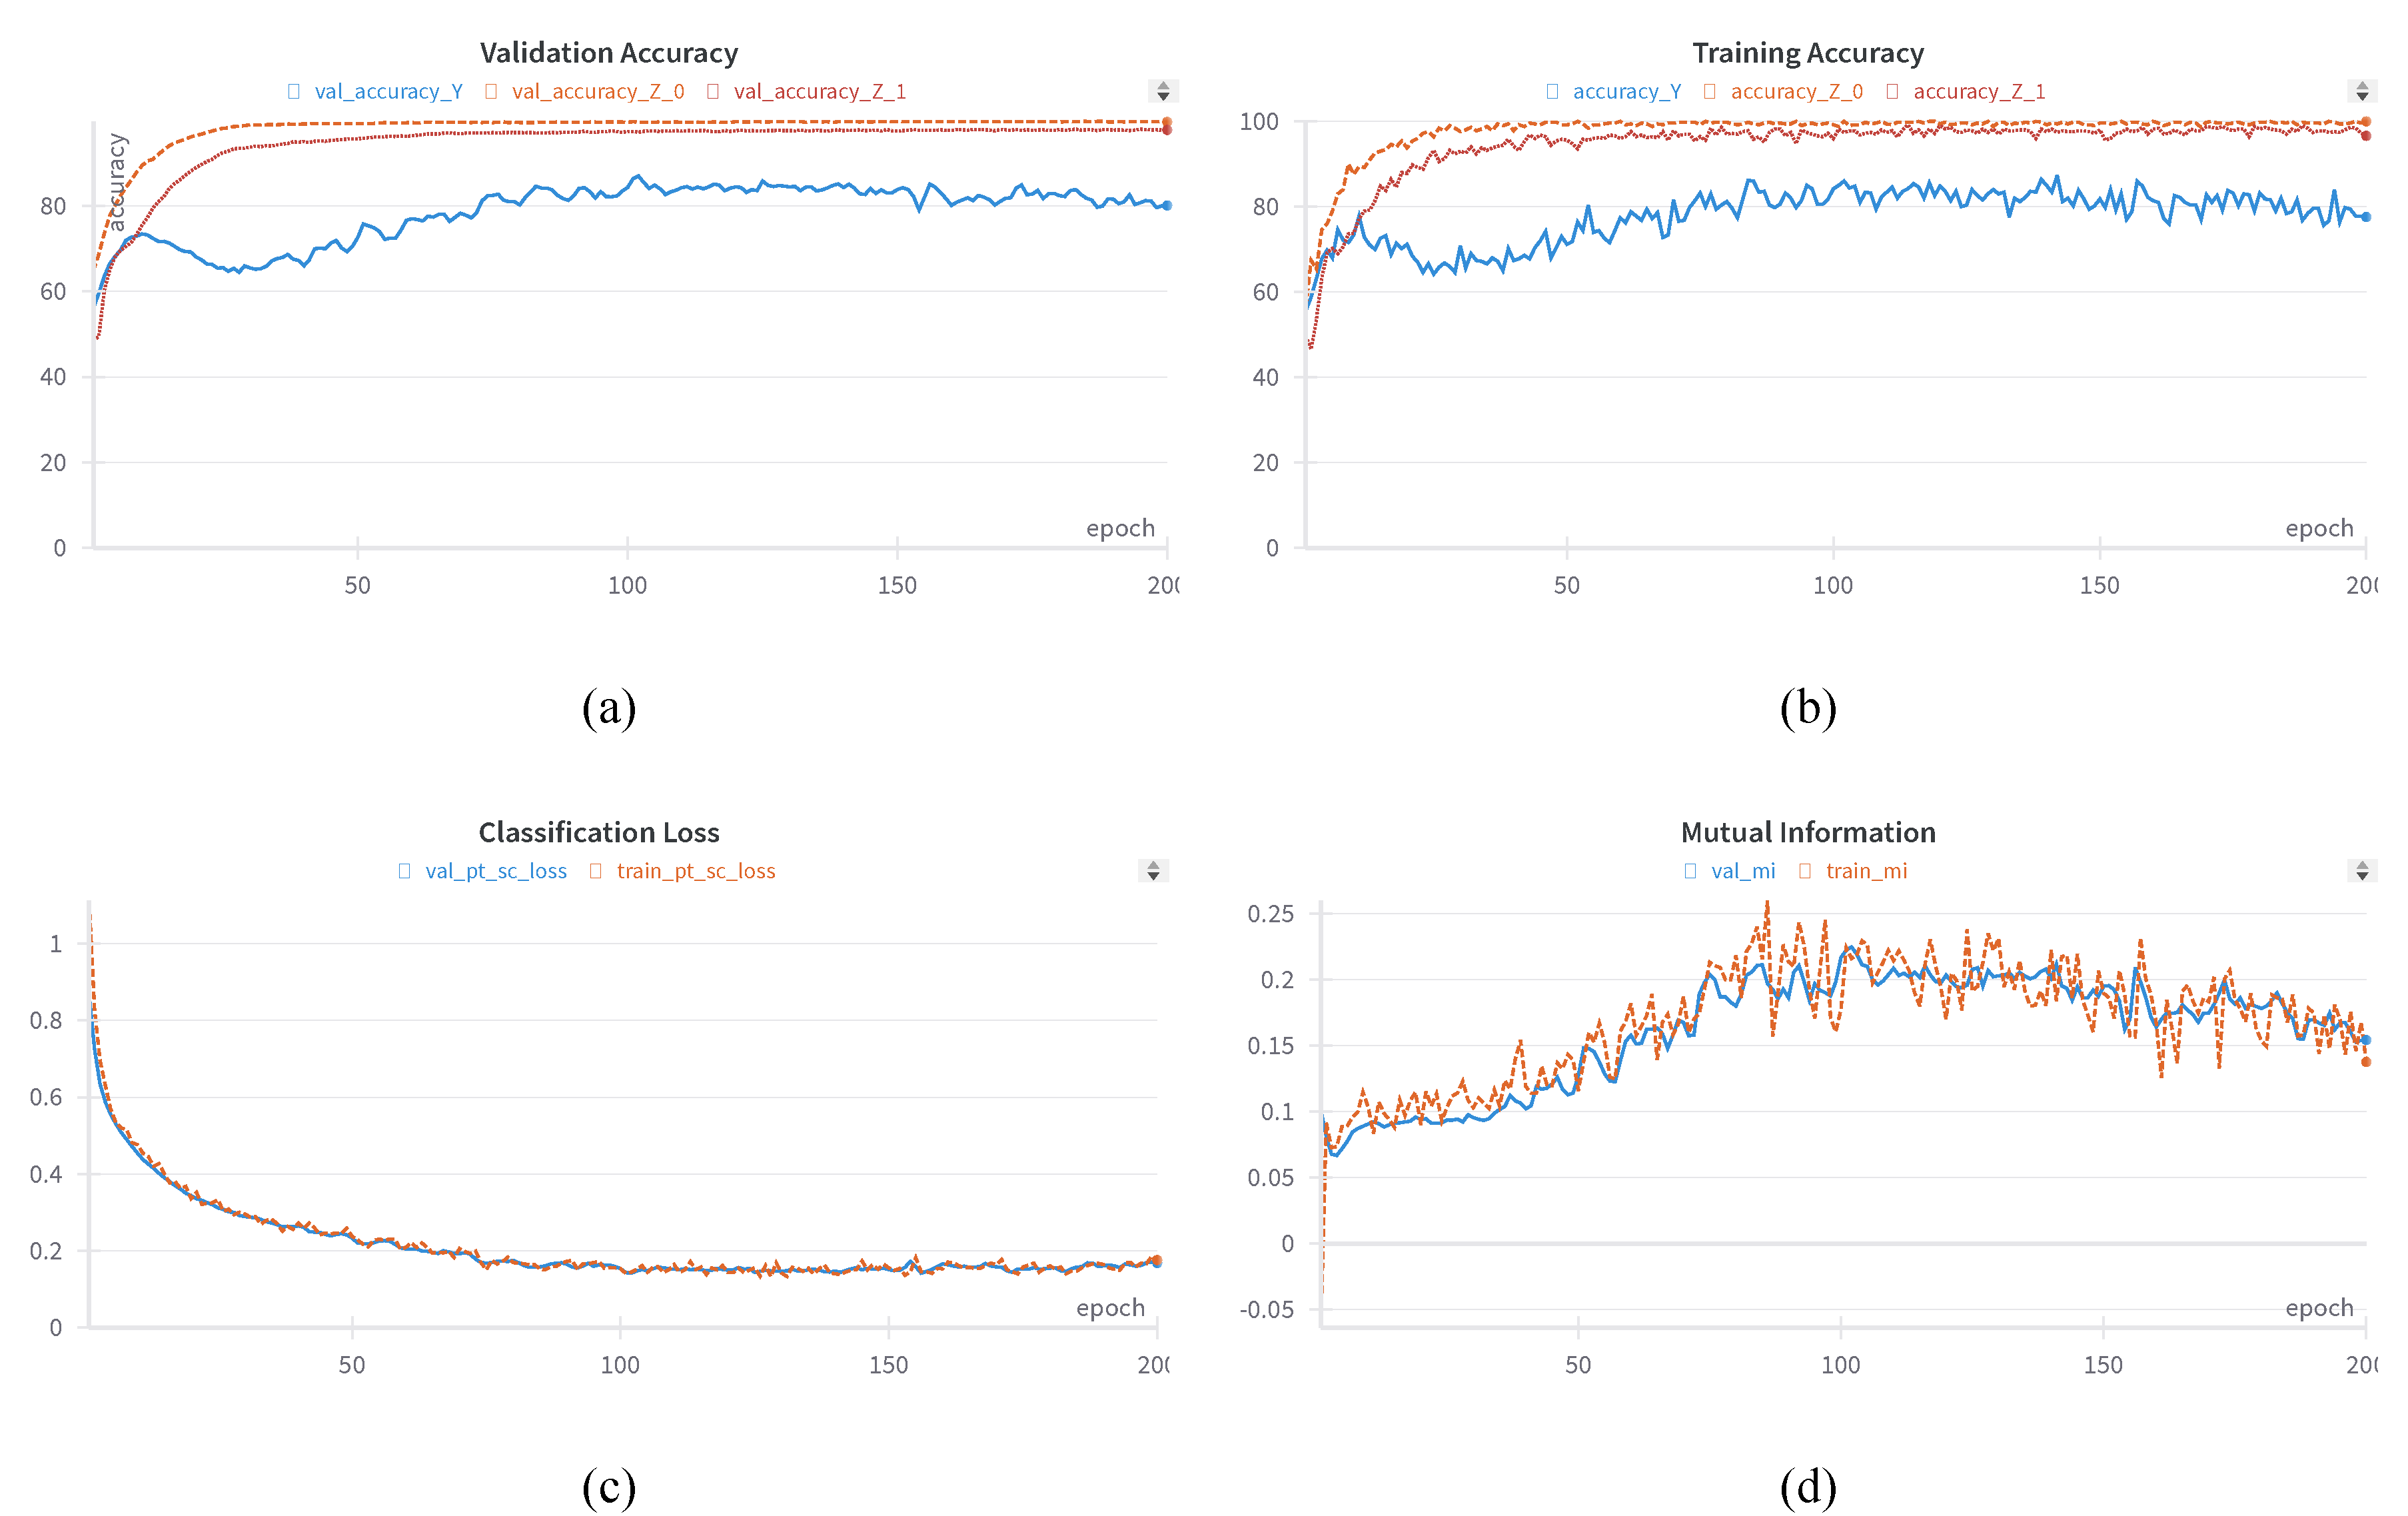
\includegraphics[width=1\linewidth]{thesis/figures/train_mnist_curve.pdf}
\caption{Morpho-MNIST MIMM model training - (a) Validation accuracy, (b) Training accuracy, (c) Classification loss, (d) Mutual information}
\label{fig:train-curve-mnist}
\end{figure}

\section{Experiments with CheXpert-Small Dataset}
This section contains the results and discussion of the experiments performed on the CheXpert-Small dataset. The experiments performed are same as those performed on the Morpho-MNIST dataset. The goal was to replicate the results on a medical dataset and test the effectiveness of MIMM model in the medical domain. The input images are chest X-rays.

The evaluation of accuracy was done on the validation, test, balanced-test dataset and the native-test dataset. The switched-labels test and t-SNE analysis were performed using the balanced-test dataset. The classification tasks used in the experiment are listed below.
\begin{itemize}
    \item [1.] Primary task, $Y$ - Classification of the presence of pleural effusion into positive for presence and negative for absence. 
    \item [2.] Spurious correlation task 1, $Z_0$ - Classification of sex of the patient, i.e. male or female. 
    \item [3.] Spurious correlation task 2, $Z_1$ - Classification of age-group of the patient, i.e. young or elder.
\end{itemize}   
\subsection{Baseline Model}
The baseline model as before has the same feature encoder and classification heads as the MIMM model used but is without the MINE models. The feature encoder used here is Densenet-121 with a modified output feature vector size of 6. The hyperparameters used for this experiment are given in table \ref{tab:chx_baseline_HP}. The training was done only for 130 epochs to prevent overfitting.
\begin{table}[H]
\centering
\begin{tabular}{|C|C|}
\hline
\textbf{Hyperparameter} & \textbf{Values} \\
\hline
$N_{epoch}$ & 130\\
$lr$ & $1\times10^{-5}$\\
$B$ & 150 \\
\hline
\end{tabular}
\caption{Training Hyperparameters-CheXpert-Small Baseline Model}
\label{tab:chx_baseline_HP}
\end{table}

\subsubsection{Accuracy}
The accuracies across various dataset splits are given in table \ref{tab:accuracy-chx_baseline}. The baseline model performs well with accuracies greater than 85\% on the validation dataset which has the same distribution as the training dataset. This performance, however, is not observed in the other datasets which have a different distribution from the training dataset. The worst primary task accuracy is 42.7\%, observed for the test dataset which has an inverted distribution when compared to the training dataset distribution.

Similar to the Morpho-MNIST experiments we can see that the balanced-test dataset shows a higher accuracy at 67.4\%, this can attributed to the absence of spurious correlations in the balanced-test dataset. This is also the case for native-test dataset with an accuracy of 60.7\%. The native dataset has a weak correlation in the same direction as that in training dataset. 

The native-test dataset, however, has a lower accuracy compared to the balanced dataset. This could be because the native-test dataset is the original test dataset of the CheXpert-Small dataset unlike the other three. The training, validation, test and balanced-test datasets are non-overlapping splits of the original training dataset of CheXpert-Small dataset.

It should also be noted that unlike in case of experiments with the Morpho-MNIST dataset, here the accuracies of the spurious correlation tasks too suffer when the distribution changes. This can be explained by the nature of these tasks which are relatively difficult to learn for the feature encoder. 

 
\begin{table}[H]
\centering 
\begin{tabular}{|l|c|c|c|c|}
\hline
\multirow{\textbf{Task}} & \multicolumn{4}{c|}{\textbf{Accuracy}} \\
\cline{2-5}
& \textbf{Val. Dataset} & \textbf{Test Dataset} & \textbf{Bal. Test Dataset} &\textbf{Native-test Dataset} \\
\hline
$Y = negative/positive$ & 90.2\% & 42.7\% & 67.4\% & 60.7\%\\
$Z_0 = male/female$     & 87.4\% & 70.3\% & 74.9\% & 77.8\%\\
$Z_1 = young/elder$     & 86.1\% & 65.3\% & 69.0\% & 69.3\%\\
\hline
\end{tabular}
\caption{Accuracy on different dataset splits - CheXpert-Small Baseline Model.}
\label{tab:accuracy-chx_baseline}
\end{table}

\subsubsection{Switched-Labels Test}
The results of the switched-labels test are given in table \ref{tab:accuracy_tasks-chx_baseline}. The feature vector of the primary task can be used to predict the labels of the spurious correlation tasks with an accuracy of $\sim65\%$. This highlights the dependence of the primary task on the spurious correlation tasks. 

Unlike the case of Morpho-MNIST dataset the predictions using the feature vector of spurious correlation task also shows a value greater than what can be achieved through random chance. This implies that baseline model utilizes spurious correlation to learn the spurious correlation tasks.
\begin{table}[H]
\centering
\begin{tabular}{|l|c|}
\hline
\textbf{Task} & \textbf{Accuracy} \\
\hline
$F_Y \rightarrow Z_0$& 65.4\%\\
$F_Y \rightarrow Z_1$ & 64.1\%\\
\hline
$F_{Z_0} \rightarrow Y$& 60.7\%\\
$F_{Z_0} \rightarrow Z_1$ & 59.1\%\\
\hline
$F_{Z_1} \rightarrow Y$& 65.8\%\\
$F_{Z_1} \rightarrow Z_0$& 62.9\%\\
\hline
\end{tabular}
\caption{Switched-Labels Test - CheXpert-Small Baseline Model.}
\label{tab:accuracy_tasks-chx_baseline}
\end{table}

\subsubsection{t-SNE}
The t-SNE plots for the feature vectors of primary task $F_Y$ coloured by the labels of the spurious correlation tasks $Z_0$ and $Z_1$ and the plots for the feature vectors of spurious correlation task $F_{Z_0}$ and $F_{Z_1}$ coloured by the labels of $Z_1$ and $Z_0$ respectively are given in the Figure \ref{fig:tsne-chx-baseline}. It can be seen that a fuzzy separation can be made for the labels in the different feature spaces illustrated. This reflects the dependencies between the classification tasks.
\begin{figure}[H]
\centering
\includegraphics[width=0.7\linewidth]{thesis/figures/tsne_chx_baseline.pdf}
\caption{t-SNE Plots for CheXpert-Small Baseline Model. (a) The feature vectors of primary task $F_Y$ coloured by labels of $Z_0$. (b) The feature vectors of primary task $F_Y$ coloured by labels of $Z_1$. (c) The feature vectors of spurious correlation task 1 $F_{Z_0}$ coloured by labels of $Z_1$. (d) The feature vectors of spurious correlation task 2 $F_{Z_1}$ coloured by labels of $Z_0$.}
\label{fig:tsne-chx-baseline}
\end{figure}

\subsection{MIMM Model with Custom Feature Encoder}
The MIMM model with a custom encoder underwent training using the hyperparameters outlined in Table \ref{tab:chx_custom_MIMM_HP}. A higher learning rate of $1 \times 10^{-3}$ was employed compared to that used for Morpho-MNIST. This adjustment was necessary to achieve satisfactory accuracy with the custom model. Without it, the model training progresses too slowly, and the accuracy plateaus at a relatively low value. However, the introduction of the MI regularization term complicates matters. The elevated learning rate hampers learning when combined with the MI regularization term.

The challenge arises from the fact that the large learning rate corresponds to a large increment of the parameters. Also during the initial training steps, the MI estimates may not accurately guide the model towards the true minima. These two factors might inadvertently steer the model away from the true minima. The curves for the training process can be seen in Figure \ref{fig:train-curve-chx_custom}, it can be seen that the loss does not decrease and therefore the accuracy never increases from 50\% of the random guess.

\begin{table}[H]
\centering
\begin{tabular}{|C|C|}
\hline
\textbf{Hyperparameter} & \textbf{Values} \\
\hline
$N_{epoch}$ & 300 \\
$lr$ & $1\times10^{-3}$\\
$N_{FE}$ & 1\\
$N_{MI}$ & 5 \\
$B$ & 200 \\
$img\_size$& $1\times300\times300$\\
$\lambda$ & 1.5  \\
\hline
\end{tabular}
\caption{CheXpert-Small MIMM Model with Custom Feature Encoder Training Hyperparameters}
\label{tab:chx_custom_MIMM_HP}
\end{table}

\begin{figure}[H]
\centering
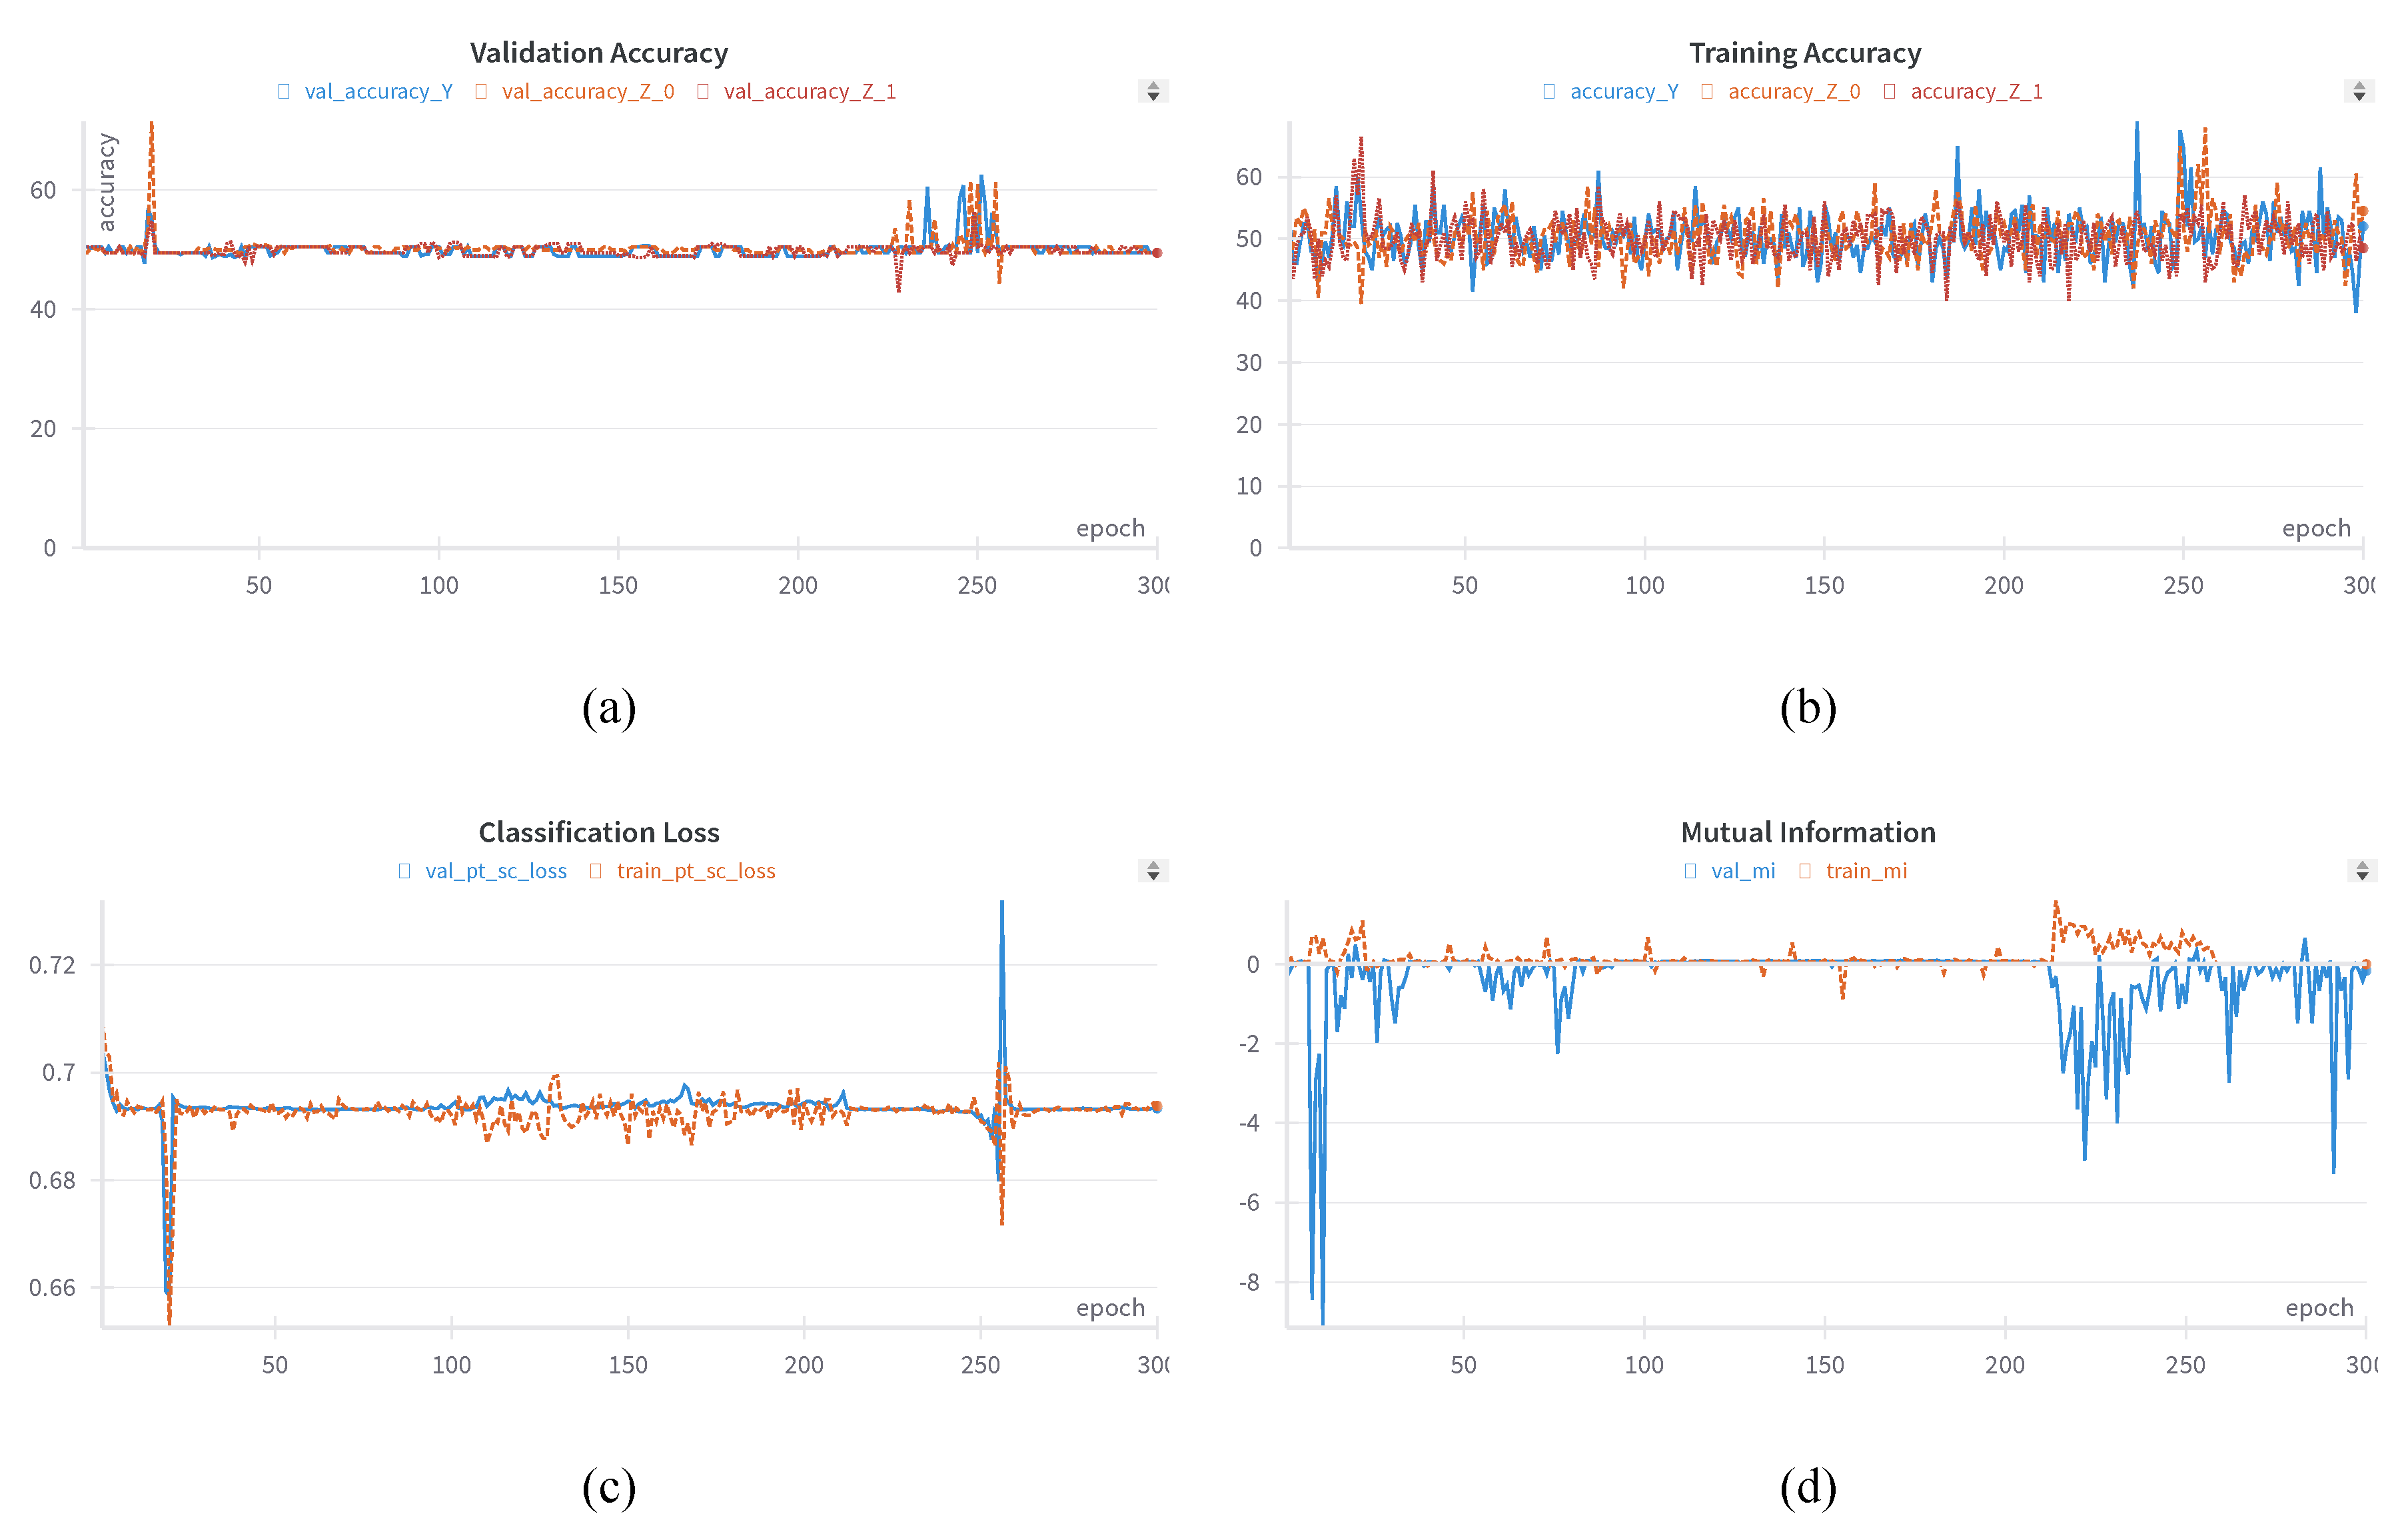
\includegraphics[width=1\linewidth]{thesis/figures/custom.pdf}
\caption{CheXpert-Small MIMM model with Custom Feature Encoder training - (a) Validation accuracy, (b) Training accuracy, (c) Classification loss, (d) Mutual information}
\label{fig:train-curve-chx_custom}
\end{figure}

\begin{table}[H]
\centering 
\begin{tabular}{|l|c|c|c|c|}
\hline
\multirow{\textbf{Task}} & \multicolumn{4}{c|}{\textbf{Accuracy}} \\
\cline{2-5}
& \textbf{Val. Dataset} & \textbf{Test Dataset} & \textbf{Bal. Test Dataset} &\textbf{Native-test Dataset} \\
\hline
$Y = negative/positive$ & 49.5\% & 49.8\% & 49.9\% & 37.8\%\\
$Z_0 = male/female$     & 49.5\% & 49.8\% & 49.9\% & 50.0\%\\
$Z_1 = young/elder$     & 49.5\% & 49.8\% & 49.9\% & 67.8\%\\
\hline
\end{tabular}
\caption{Accuracy on different dataset splits - CheXpert-Small MIMM Model with custom feature encoder.}
\label{tab:accuracy-chx_custom}
\end{table}

\subsection{MIMM Model with Densenet-121 Feature Encoder}
This MIMM model used for the experiments here employs the Densenet-121 architecture as the feature encoder. The MI estimate is used as a regularisation term and hyperparameters used for the experiment are given in the table \ref{tab:chx_dense_MIMM_HP}. An additional hyperparameter for image size is also provided to rescale the input images. The images are downscaled due to memory constraints. The experiments are the same as those performed for the Morpho-MNIST dataset and are listed below. 

\begin{itemize}
    \item [E.1.] Training without adaptive scaling and corrected MI gradients.
    \item [E.2.] Training with both adaptive scaling and corrected MI gradients.    
    \item [E.3.] Training with adaptive scaling and without the corrected MI gradients.
    \item [E.4.] Training without adaptive scaling and with the corrected MI gradients.
\end{itemize}

\begin{table}[H]
\centering
\begin{tabular}{|C|C|}
\hline
\textbf{Hyperparameter} & \textbf{Values} \\
\hline
$N_{epoch}$ & 300 \\
$lr$ & $1\times10^{-5}$\\
$N_{FE}$ & 1\\
$N_{MI}$ & 5 \\
$B$ & 150 \\
$img\_size$& $3\times96\times96$\\
$\lambda$ & 1.5  \\
\hline
\end{tabular}
\caption{CheXpert-Small MIMM model with Densenet-121 Feature Encoder training Hyperparameters}
\label{tab:chx_dense_MIMM_HP}
\end{table}

\subsubsection{Accuracy}
The tables below showcase the accuracy obtained for experiments E.1-E.4. The accuracy of the primacy task for the test dataset has improved to a value greater than 65\% from the 42.7\% of the baseline model. This improvement can also be seen in balanced-test and native-test datasets. The primary task accuracy on the test dataset is greater than 70\% when adaptive scaling is used during training, hence illustrating its ability to prevent over-regularisation and thus helping the model to balance between classification loss and MI loss. 

The validation accuracy, as expected from the Morpho-MNIST experiments, falls compared to that offered by the baseline model. This is because the model no longer utilizes the spurious correlation from the training dataset for predicting against similar correlations in the validation dataset. However, this accuracy still remains comparable to the accuracy on test dataset.


\begin{table}[H]
\centering
\begin{tabular}{|l|c|c|c|c|}
\hline
\multirow{\textbf{Task}} & \multicolumn{4}{c|}{\textbf{Accuracy}} \\
\cline{2-5}
& \textbf{Val. Dataset} & \textbf{Test Dataset} & \textbf{Bal. Test Dataset} &\textbf{Native-test Dataset} \\
\hline
$Y = negative/positive$ & 81.0\% & 65.9\% & 75.2\% & 67.8\%\\
$Z_0 = male/female$     & 77.2\% & 78.2\% & 75.8\% & 74.3\%\\
$Z_1 = young/elder$     & 69.7\% & 67.9\% & 70.6\% & 66.4\%\\
\hline
\end{tabular}
\caption{E.1. Accuracy on Different Datasets - CheXpert-Small MIMM model trained without adaptive scaling and corrected MI gradients.}
\label{tab:accuracy-chx_MIMM_noada_nocorr}
\end{table}

\begin{table}[H]
\centering
\begin{tabular}{|l|c|c|c|c|}
\hline
\multirow{\textbf{Task}} & \multicolumn{4}{c|}{\textbf{Accuracy}} \\
\cline{2-5}
& \textbf{Val. Dataset} & \textbf{Test Dataset} & \textbf{Bal. Test Dataset} &\textbf{Native-test Dataset} \\
\hline
$Y = negative/positive$ & 76.4\% & 71.9\% & 72.3\% & 66.4\%\\
$Z_0 = male/female$     & 82.0\% & 76.7\% & 81.0\% & 79.3\%\\
$Z_1 = young/elder$     & 79.5\% & 69.4\% & 74.8\% & 73.6\%\\
\hline
\end{tabular}
\caption{E.2. Accuracy on Different Datasets - CheXpert-Small MIMM model trained with both adaptive scaling and corrected MI gradients.}
\label{tab:accuracy-chx_MIMM_ada_corr}
\end{table}

\begin{table}[H]
\centering
\begin{tabular}{|l|c|c|c|c|}
\hline
\multirow{\textbf{Task}} & \multicolumn{4}{c|}{\textbf{Accuracy}} \\
\cline{2-5}
& \textbf{Val. Dataset} & \textbf{Test Dataset} & \textbf{Bal. Test Dataset} &\textbf{Native-test Dataset} \\
\hline
$Y = negative/positive$ & 72.8\% & 72.1\% & 73.3\% & 65.7\%\\
$Z_0 = male/female$     & 79.2\% & 81.3\% & 81.5\% & 85.0\%\\
$Z_1 = young/elder$     & 73.6\% & 69.9\% & 74.6\% & 69.3\%\\
\hline
\end{tabular}
\caption{E.3. Accuracy on Different Datasets - CheXpert-Small MIMM model trained with adaptive scaling and without corrected MI gradients.}
\label{tab:accuracy-chx_MIMM_ada_nocorr}
\end{table}

\begin{table}[H]
\centering
\begin{tabular}{|l|c|c|c|c|}
\hline
\multirow{\textbf{Task}} & \multicolumn{4}{c|}{\textbf{Accuracy}} \\
\cline{2-5}
& \textbf{Val. Dataset} & \textbf{Test Dataset} & \textbf{Bal. Test Dataset} &\textbf{Native-test Dataset} \\
\hline
$Y = negative/positive$ & 78.9\% & 68.1\% & 73.8\% & 66.4\%\\
$Z_0 = male/female$     & 79.5\% & 77.2\% & 78.1\% & 82.1\%\\
$Z_1 = young/elder$     & 69.5\% & 70.9\% & 70.3\% & 75.0\%\\
\hline
\end{tabular}
\caption{E.4. Accuracy on Different Datasets - CheXpert-Small MIMM model trained without adaptive scaling and with corrected MI gradients.}
\label{tab:accuracy-chx_MIMM_noada_corr}
\end{table}

\subsubsection{Switched-Labels Test}
The results for the switched test is laid out in the tables \ref{tab:accuracy_tasks-chxMIMM_noada_nocorr}-\ref{tab:accuracy_tasks-chxMIMM_noada_corr}. The MIMM model reduces the accuracy of predicting the switched labels from $\sim65\%$ in the baseline model to $\sim50\%$. Since the accuracies for the switched-label tasks are near to that which can be acquired through random chance, it can be said that MIMM model has been successful at learning the tasks without relying on the spurious correlation. 

\begin{table}[H]
\centering
\begin{minipage}{.45\linewidth}
\centering
\begin{tabular}{|l|c|}
\hline
\textbf{Task} & \textbf{Accuracy} \\
\hline
$F_Y \rightarrow Z_0$ & 55.3\% \\
$F_Y \rightarrow Z_1$ & 56.2\% \\
\hline
$F_{Z_0} \rightarrow Y$ & 48.7\% \\
$F_{Z_0} \rightarrow Z_1$ & 49.6\% \\
\hline
$F_{Z_1} \rightarrow Y$ & 48.7\% \\
$F_{Z_1} \rightarrow Z_0$ & 48.7\% \\
\hline
\end{tabular}
\caption{E.1. Switched-Labels Test - CheXpert-Small MIMM model trained without adaptive scaling and corrected MI gradients.}
\label{tab:accuracy_tasks-chxMIMM_noada_nocorr}
\end{minipage}%
\hfill
\begin{minipage}{.45\linewidth}
\centering
\begin{tabular}{|l|c|}
\hline
\textbf{Task} & \textbf{Accuracy} \\
\hline
$F_Y \rightarrow Z_0$ & 47.7\% \\
$F_Y \rightarrow Z_1$ & 49.5\% \\
\hline
$F_{Z_0} \rightarrow Y$ & 50.9\% \\
$F_{Z_0} \rightarrow Z_1$ & 49.4\% \\
\hline
$F_{Z_1} \rightarrow Y$ & 54.5\% \\
$F_{Z_1} \rightarrow Z_0$ & 51.5\% \\
\hline
\end{tabular}
\caption{E.2. Switched-Labels Test - CheXpert-Small MIMM model trained with both adaptive scaling and corrected MI gradients.}
\label{tab:accuracy_tasks-chxMIMM_ada_corr}
\end{minipage}%
\end{table}

\vspace{-2.5cm}

\begin{table}[H]
\centering
\begin{minipage}{.45\linewidth}
\centering
\begin{tabular}{|l|c|}
\hline
\textbf{Task} & \textbf{Accuracy} \\
\hline
$F_Y \rightarrow Z_0$ & 49.5\% \\
$F_Y \rightarrow Z_1$ & 49.9\% \\
\hline
$F_{Z_0} \rightarrow Y$ & 50.6\% \\
$F_{Z_0} \rightarrow Z_1$ & 48.9\% \\
\hline
$F_{Z_1} \rightarrow Y$ & 54.3\% \\
$F_{Z_1} \rightarrow Z_0$ & 50.6\% \\
\hline
\end{tabular}
\caption{E.3. Switched-Labels Test - CheXpert-Small MIMM model trained with adaptive scaling and without corrected MI gradients.}
\label{tab:accuracy_tasks-chxMIMM_ada_nocorr}
\end{minipage}%
\hfill
\begin{minipage}{.45\linewidth}
\centering
\begin{tabular}{|l|c|}
\hline
\textbf{Task} & \textbf{Accuracy} \\
\hline
$F_Y \rightarrow Z_0$ & 51.2\% \\
$F_Y \rightarrow Z_1$ & 53.4\% \\
\hline
$F_{Z_0} \rightarrow Y$ & 50.2\% \\
$F_{Z_0} \rightarrow Z_1$ & 50.1\% \\
\hline
$F_{Z_1} \rightarrow Y$ & 50.6\% \\
$F_{Z_1} \rightarrow Z_0$ & 48.8\% \\
\hline
\end{tabular}
\caption{E.4. Switched-Labels Test - CheXpert-Small MIMM model trained without adaptive scaling and with corrected MI gradients.}
\label{tab:accuracy_tasks-chxMIMM_noada_corr}
\end{minipage}%
\end{table}


\subsubsection{t-SNE Plots}
The t-SNE plots for experiments E.1-E.4 are given in the figures in the next page. It can be seen that the labels are inseparable in t-SNE plots. The inseparability of $Z_0$ and $Z_1$ labels from the plots of $F_{Y} \rightarrow Z_0$ and $F_{Y} \rightarrow Z_1$, i.e. the plots (a) and (b), show that the influence of demographics sex and age on the detection of pleural effusion has been removed. It can also be seen that the proposed model was also able to remove the relationship between sex and age, i.e. the spurious correlation variables. 

\nextpage


\begin{figure}[H]
\begin{center}
\includegraphics[width=0.7\linewidth]{thesis/figures/tsne_chx_noada_nocorr.pdf}
\caption{E.1. t-SNE Plots for CheXpert-Small MIMM model without adaptive scaling and corrected MI gradients.}
\includegraphics[width=0.7\linewidth]{thesis/figures/tsne_chx_ada_corr.pdf}
\caption{E.2. t-SNE Plots for CheXpert-Small MIMM model with both adaptive scaling and corrected MI gradients.}
\end{center}
\end{figure}

\begin{figure}[H]
\centering
\includegraphics[width=0.7\linewidth]{thesis/figures/tsne_chx_ada_nocorr.pdf}
\caption{E.3. t-SNE Plots for CheXpert-Small MIMM model with adaptive scaling and without corrected MI gradients.}
\includegraphics[width=0.7\linewidth]
{thesis/figures/tsne_chx_noada_corr.pdf}
\caption{E.4. t-SNE Plots for CheXpert-Small MIMM model without adaptive scaling and with corrected MI gradients.}
\caption*{\textbf{t-SNE Plots - }(a) The feature vectors of primary task $F_Y$ coloured by labels of $Z_0$. (b) The feature vectors of primary task $F_Y$ coloured by labels of $Z_1$. (c) The feature vectors of spurious correlation task 1 $F_{Z_0}$ coloured by labels of $Z_1$. (d) The feature vectors of spurious correlation task 2 $F_{Z_1}$ coloured by labels of $Z_0$.}
\end{figure}

\subsubsection{Model Training Analysis}

The training curves are presented in Figure \ref{fig:train-curve-chx}. The classification loss curve is monitored and the training was stopped when overfitting was noticed. The MI as in case of Morpho-MNIST dataset spikes first and then is controlled through the regularisation term. It can be observed from the accuracy curves that the spurious correlation tasks, i.e. sex and age, were relatively more difficult to learn compared to the primary task of pleural effusion. Although this was the case the spuriously correlated tasks still had a significant influence on the primary task while training with the baseline model while the MIMM model evaded this issue.

\begin{figure}[H]
\centering
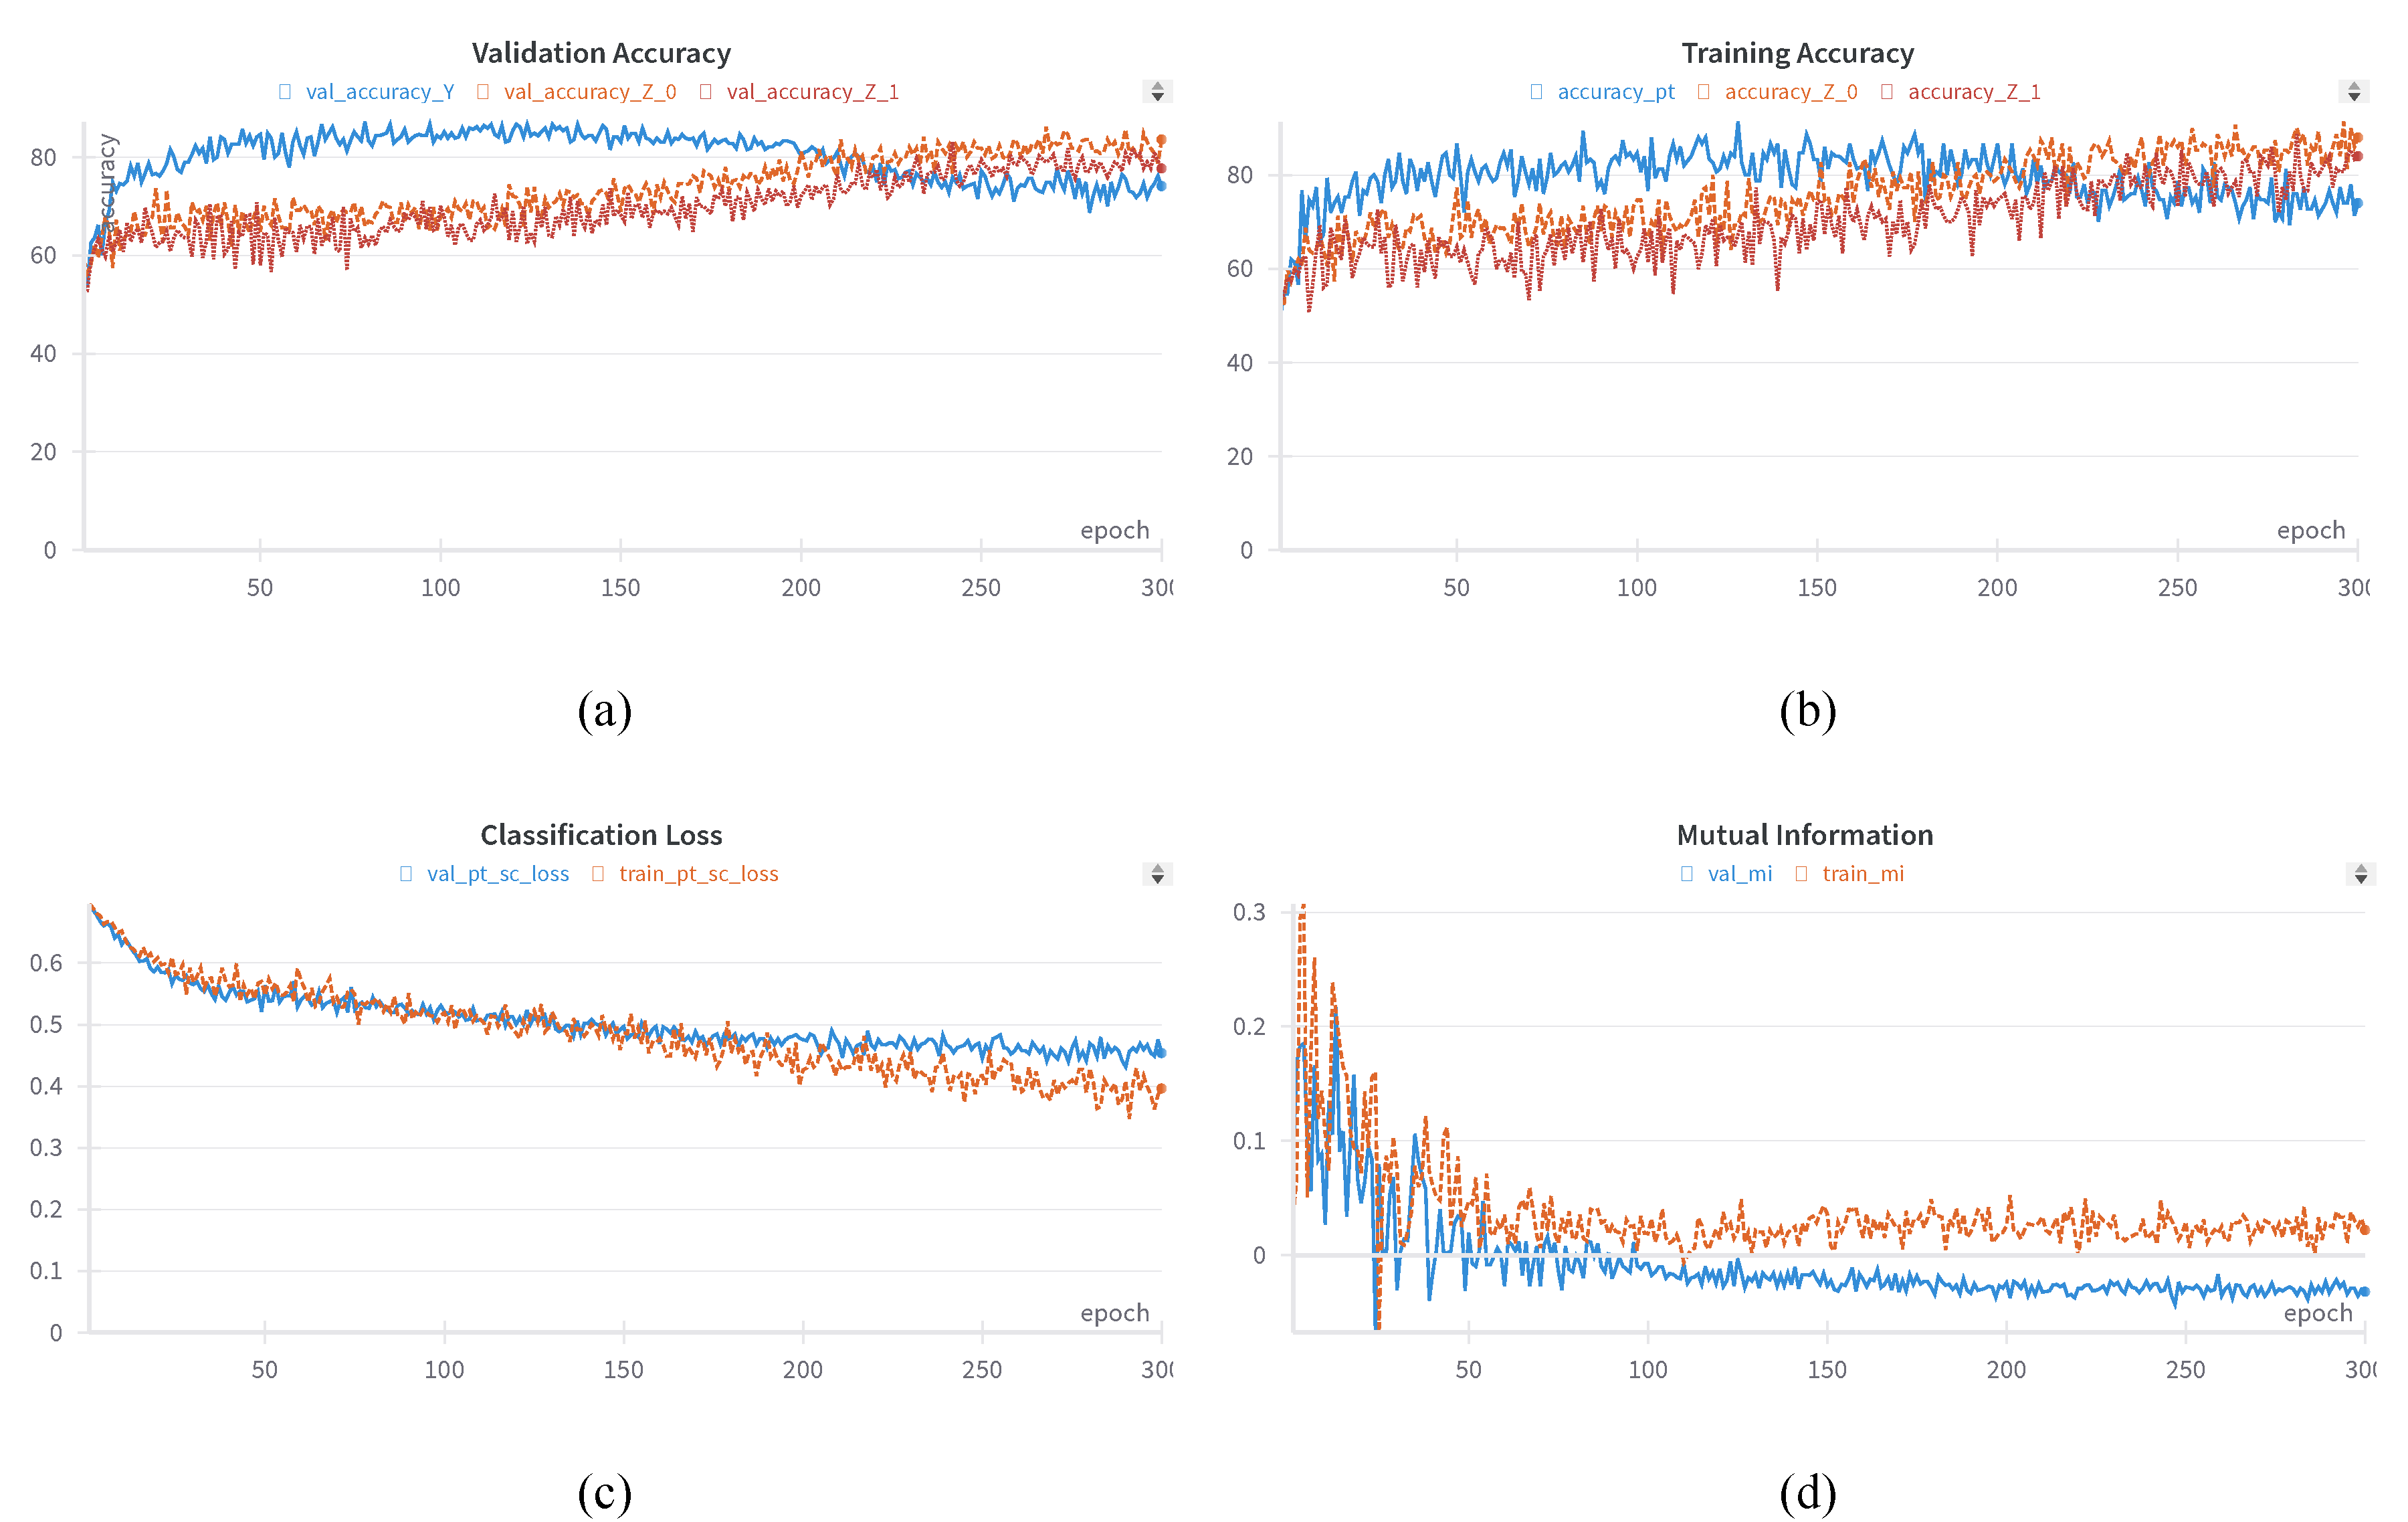
\includegraphics[width=1\linewidth]{thesis/figures/train_chx_curve.pdf}
\caption{CheXpert-Small MIMM model with Densenet-121 Feature Encoder training - (a) Validation accuracy, (b) Training accuracy, (c) Classification loss, (d) Mutual information}
\label{fig:train-curve-chx}
\end{figure}


\chapter{Conclusion}
The research thesis delved into learning causal relationships from data in the presence of multiple spurious correlations. A thorough examination of causal inference and counterfactual invariance was conducted to establish a foundation for understanding the complexities of causal relationships and the limitations of relying solely on correlations for inference. The causal structure of two datasets, Morpho-MNIST and CheXpert-Small, was analyzed and the MIMM, originally proposed by Fay et al., was extended to address the challenge posed by multiple correlations.

The proposed model successfully learned the causal structure of the data while circumventing the spurious correlations inherent within. An exploration of the MINE model was conducted to understand its weaknesses, prompting the implementation of adaptive scaling within the MIMM loss function's MI regularization term. This adjustment proved to be useful in preventing the model from fixating on the regularization term, thus striking a balance between enhancing classification accuracy and mitigating the influence of spurious correlations. Additionally, the effects of utilizing corrected gradients for MI were investigated through experiments. It was observed that the impact of employing this technique was negligible. A plausible explanation, contingent upon how MI was calculated, was also provided.

The proposed methodology although successful has areas of improvement where future work is possible. The implementation of adaptive scaling requires additional gradient calculation which increases the computational cost. Moreover, the current approach necessitates the calculation of MI between all possible combinations of spurious correlation tasks, which is also computationally demanding. Additionally, the model assumes prior knowledge of the spuriously correlated tasks, highlighting the need for further research in the direction of causal discovery algorithms \cite{10162210}.






 
\appendix
\chapter{Algorithms}
\section{Algorithm for mutual information neural estimation} 
\vspace{-0.4cm}
\begin{algorithm}[H]
\caption{MINE - Algorithm for mutual information neural estimation \cite{DBLP:journals/corr/abs-1801-04062}}
\begin{algorithmic}[0]
\State $\theta \gets$ initialize network parameters
\Repeat
\State Draw $B$ minibatch samples from the joint distribution: $(y^{(1)}, z^{(1)}), \ldots, (y^{(b)}, z^{(b)}) \sim \mathbb{P}_{YZ}$
\State Generate $B \times (B-1)$ shuffled samples for the independent distribution $(y', z') \sim \mathbb{P}_{Y} \otimes \mathbb{P}_{Z}$.
\State Evaluate the lower-bound: 
    \begin{center}
     \Statex $\mathcal{V}(\theta) \gets \frac{1}{B} \sum_{i=1}^{B} T_{\theta}(y^{(i)},z^{(i)}) - \log\left(\frac{1}{B\times(B-1)} \sum_{i=1}^{B\times(B-1)} e^{T_{\theta}(y',z')\right)$   
    \end{center}     
\State Evaluate the gradients: 
    \begin{center}
    \Statex $\widehat{G}(\theta) \gets \widehat{\nabla}_{\theta} \mathcal{V}(\theta)$
    \end{center}  
\State Update the statistics network parameters: 
    \begin{center}
    \Statex $\theta \gets \theta + \widehat{G}(\theta)$
    \end{center}  
\Until{convergence}
\end{algorithmic}
\end{algorithm}

\section{Steps for creating confounded Morpho-MNIST dataset}
\begin{algorithm}[H] 
\caption{Steps for creating confounding in the Morpho-MNIST dataset}
\label{alg:create_morpho}
\begin{algorithmic}[1]
\State Load the 'Global' Morpho-MNIST dataset
\State Load the 'Global' training dataset for creating training dataset or the test dataset for validation, test and balanced-test.
\State Set the primary task labels as low (0) and high (1):
\Statex \hspace{\algorithmicindent} Primary task ($Y$): \hspace{0.5cm} 0-4 $\rightarrow$ 0 \hspace{0.5cm} 5-9 $\rightarrow$ 1
\State Remove the plain images
\State Set the perturbation (thin/thick) labels:
\Statex \hspace{\algorithmicindent} Spurious correlation task-1 ($Z_0$): \hspace{0.5cm} thin $\rightarrow$ 0 \hspace{0.5cm} thick $\rightarrow$ 1
\State Create the spurious correlation through sampling according to specified ratios in table \ref{tab:cfr_ratios}.
\State Shuffle the dataset 
\State Create the spurious correlation $Z_1$ through selective rotation by $90^\circ$ according to specified ratios in table \ref{tab:cfr_ratios}:
\Statex \hspace{\algorithmicindent} spurious correlation task-2 ($Z_1$): \hspace{0.5cm} not-rotated $\rightarrow$ 0 \hspace{0.5cm} rotated $\rightarrow$ 1
\end{algorithmic}
\end{algorithm}

\section{Steps for creating confounded CheXpert-Small dataset}
\begin{algorithm}[H]
\caption{Steps for creating confounded CheXpert-Small dataset}
\label{alg:create_chxpert}
\begin{algorithmic}[1]
\State Load the CheXpert-Small Dataset 
\State Split the original training dataset in the ratio 74.7:8.3:17 for training:validation:test dataset. 
\State Map the sex of the patients to 0 and 1:
\Statex \hspace{\algorithmicindent} Spurious correlation task-1 ($Z_0$): \hspace{0.5cm} Male $\rightarrow$ 0 \hspace{0.5cm} Female $\rightarrow$ 1
\State Binarize the age of the patients to 0 and 1:
\Statex \hspace{\algorithmicindent} Spurious correlation task-2 ($Z_1$): \hspace{0.5cm} $<=50$ $\rightarrow$ 0 \hspace{0.5cm} $>=60$ $\rightarrow$ 1
\State Remove lateral views.
\State Remove PA views.
\State Remove data instances where pleural effusion is not labelled.
\State Remove data instances where pleural effusion label is uncertain.
\State Calculate the ratio of each combination of labels in the dataset using table \ref{tab:cfr_ratios}. Step omitted for native-test dataset.
\State Sample from the dataset according to this ratio to create correlation in the dataset.Step omitted for native-test dataset.
\end{algorithmic}
\end{algorithm}

\section{Algorithm for training MIMM model}
\begin{algorithm}[H]
\caption{MIMM Training}
\label{alg:training}
\begin{algorithmic}[1]
\State \textbf{Input:} Training data loader $trainLoader$ and Validation data loader $valLoader$.
\State Initialize ADAM optimizers for classification models and MINE model
\For{$epoch$ \textbf{in} $1$ \textbf{to} $N_{epochs}$}:
    \For{$step$ \textbf{in} $num\_steps\_per\_epoch$}
        \For{$batches$ \textbf{in} $N_{FE}$}
            \State Freeze the parameters of Mutual Information Models
            \State Estimate MI using the current state of MINE models and the classification loss using the current state if feature encoder.
            \State Train Feature Encoder and Primary Task Models by minimizing $\mathcal{L}_{MIMM}$ and backpropagating through both of them.
        \EndFor
        \For{$batches$ \textbf{in} $N_{MI}$}
            \State Freeze the parameters of Feature Encoder and Primary Task Models
            \State Train Statistics network by maximizing the MI output of MINE model and backpropagating through the MINE models. 
        \EndFor
    \EndFor
    \State Evaluate models on validation set
\EndFor

\State Save the Models for testing and t-SNE plots.

\end{algorithmic}
\end{algorithm}


\chapter{Models}
\section{Morpho-MNIST Custom Feature Encoder}
\vspace{-0.5cm}
\begin{table}[H]
\caption{Model Summary - Morpho-MNIST Custom Model}
\centering
\begin{tabular}{|l|l|l|}
\hline
Layer & Output Shape & Param \# \\
\hline
FeatureEncoderNetwork & [1, 6] & -- \\
\hline
\quad Sequential & [1, 16, 4, 4] & -- \\
\quad\quad Conv2d & [1, 6, 26, 26] & 60 \\
\quad\quad ReLU & [1, 6, 26, 26] & -- \\
\quad\quad MaxPool2d & [1, 6, 13, 13] & -- \\
\quad\quad Conv2d & [1, 16, 11, 11] & 880 \\
\quad\quad ReLU & [1, 16, 11, 11] & -- \\
\quad\quad Conv2d & [1, 16, 9, 9] & 2,320 \\
\quad\quad ReLU & [1, 16, 9, 9] & -- \\
\quad\quad MaxPool2d & [1, 16, 4, 4] & -- \\
\hline
\quad Linear & [1, 256] & 65,792 \\
\quad Linear & [1, 6] & 1,542 \\
\hline
\end{tabular}
\label{tab:model_summary}
\end{table}

\begin{table}[ht]
\caption{Model Details}
\centering
\begin{tabular}{|l|l|}
\hline
Total params & 70,594 \\
\hline
Trainable params & 70,594 \\
\hline
Non-trainable params & 0 \\
\hline
Total mult-adds (M) & 0.40 \\
\hline
\end{tabular}
\label{tab:model_details}
\end{table}


\section{Densenet-121 feature encoder}
\vspace{-0.5cm}
\begin{table}[H]
\caption{Model Summary - Densenet-121}
\centering
\begin{tabular}{|l|l|l|}
\hline
Layer & Output Shape & Param \# \\
\hline
chXception & [1, 6] & -- \\
\hline
\quad DenseNet & [1, 6] & -- \\
\quad\quad Sequential & [1, 1024, 3, 3] & -- \\
\quad\quad\quad Conv2d & [1, 64, 48, 48] & 9,408 \\
\quad\quad\quad BatchNorm2d & [1, 64, 48, 48] & 128 \\
\quad\quad\quad ReLU & [1, 64, 48, 48] & -- \\
\quad\quad\quad MaxPool2d & [1, 64, 24, 24] & -- \\
\quad\quad\quad DenseBlock & [1, 256, 24, 24] & 335,040 \\
\quad\quad\quad Transition & [1, 128, 12, 12] & 33,280 \\
\quad\quad\quad DenseBlock & [1, 512, 12, 12] & 919,680 \\
\quad\quad\quad Transition & [1, 256, 6, 6] & 132,096 \\
\quad\quad\quad DenseBlock & [1, 1024, 6, 6] & 2,837,760 \\
\quad\quad\quad Transition & [1, 512, 3, 3] & 526,336 \\
\quad\quad\quad DenseBlock & [1, 1024, 3, 3] & 2,158,080 \\
\quad\quad\quad BatchNorm2d & [1, 1024, 3, 3] & 2,048 \\
\quad\quad Linear & [1, 6] & 6,150 \\
\hline
\end{tabular}
\label{tab:densenet}
\end{table}
\vspace{-0.5cm}
\begin{table}[ht]
\caption{Model Details - Densenet-121}
\centering
\begin{tabular}{|l|l|}
\hline
Total params & 6,960,006 \\
\hline
Trainable params & 6,960,006 \\
\hline
Non-trainable params & 0 \\
\hline
Total mult-adds (M) & 520.46 \\
\hline
\end{tabular}
\label{tab:model_details_dense}
\end{table}
\section{CheXpert Custom Feature Encoder}
\vspace{-0.5cm}
\begin{table}[ht]
\caption{Model Summary - CheXpert Custom Model}
\centering
\begin{tabular}{|l|l|l|}
\hline
Layer & Output Shape & Param \# \\
\hline
MedicalFeatureEncoder & [1, 6] & -- \\
\hline
\quad Sequential & [1, 128, 1, 1] & -- \\
\quad\quad Conv2d & [1, 3, 298, 298] & 30 \\
\quad\quad ReLU & [1, 3, 298, 298] & -- \\
\quad\quad Conv2d & [1, 6, 296, 296] & 168 \\
\quad\quad ReLU & [1, 6, 296, 296] & -- \\
\quad\quad Conv2d & [1, 8, 294, 294] & 440 \\
\quad\quad ReLU & [1, 8, 294, 294] & -- \\
\quad\quad Conv2d & [1, 8, 292, 292] & 584 \\
\quad\quad ReLU & [1, 8, 292, 292] & -- \\
\quad\quad MaxPool2d & [1, 8, 97, 97] & -- \\
\quad\quad BatchNorm2d & [1, 8, 97, 97] & 16 \\
\quad\quad Conv2d & [1, 16, 95, 95] & 1,168 \\
\quad\quad ReLU & [1, 16, 95, 95] & -- \\
\quad\quad Conv2d & [1, 16, 93, 93] & 2,320 \\
\quad\quad ReLU & [1, 16, 93, 93] & -- \\
\quad\quad Conv2d & [1, 16, 91, 91] & 2,320 \\
\quad\quad ReLU & [1, 16, 91, 91] & -- \\
\quad\quad Conv2d & [1, 16, 89, 89] & 2,320 \\
\quad\quad ReLU & [1, 16, 89, 89] & -- \\
\quad\quad MaxPool2d & [1, 16, 29, 29] & -- \\
\quad\quad BatchNorm2d & [1, 16, 29, 29] & 32 \\
\quad\quad Conv2d & [1, 32, 27, 27] & 4,640 \\
\quad\quad ReLU & [1, 32, 27, 27] & -- \\
\quad\quad Conv2d & [1, 32, 25, 25] & 9,248 \\
\quad\quad ReLU & [1, 32, 25, 25] & -- \\
\quad\quad Conv2d & [1, 32, 23, 23] & 9,248 \\
\quad\quad ReLU & [1, 32, 23, 23] & -- \\
\quad\quad MaxPool2d & [1, 32, 7, 7] & -- \\
\quad\quad BatchNorm2d & [1, 32, 7, 7] & 64 \\
\quad\quad Conv2d & [1, 64, 5, 5] & 18,496 \\
\quad\quad ReLU & [1, 64, 5, 5] & -- \\
\quad\quad Conv2d & [1, 128, 3, 3] & 73,856 \\
\quad\quad ReLU & [1, 128, 3, 3] & -- \\
\quad\quad AvgPool2d & [1, 128, 1, 1] & -- \\
\hline
\quad Sequential & [1, 6] & -- \\
\quad\quad Linear & [1, 64] & 8,256 \\
\quad\quad ReLU & [1, 64] & -- \\
\quad\quad Linear & [1, 32] & 2,080 \\
\quad\quad ReLU & [1, 32] & -- \\
\quad\quad Linear & [1, 12] & 396 \\
\quad\quad ReLU & [1, 12] & -- \\
\quad\quad Linear & [1, 6] & 78 \\
\hline
\end{tabular}
\label{tab:ChX_custom}
\end{table}
\vspace{-0.5cm}
\begin{table}[H]
\caption{Model Details - CheXpert Custom Model}
\centering
\begin{tabular}{|l|l|}
\hline
Total params & 135,760 \\
\hline
Trainable params & 135,760 \\
\hline
Non-trainable params & 0 \\
\hline
Total mult-adds (M) & 188.60 \\
\hline
\end{tabular}
\label{tab:model_details_chx}
\end{table}

% -------------------> end writing here <------------------------
% *****************************************************************
\listoffigures
\listoftables

\ifthenelse{\equal{\doclang}{german}}{
	\bibliographystyle{IEEEtran_ISSger}
}{
	\bibliographystyle{IEEEtran_ISS}
}
\bibliography{refs}

% *****************************************************************
%% Additional page with Declaration ("Eidesstattliche Erklrung");
%% completed automatically
\begin{titlepage}
      \vfill
      \LARGE \ifthenelse{\equal{\doclang}{german}}{\textbf{Erkl\"arung}}{\textbf{Declaration}}
      \vfill

      \ifthenelse{\equal{\doclang}{german}}{
         Hiermit erkl\"are ich, dass ich diese Arbeit selbstst\"andig verfasst und keine anderen als die angegebenen
         Quellen und Hilfsmittel benutzt habe.
      }
      {
         Herewith, I declare that I have developed and written the enclosed thesis entirely by myself and that I have not used sources or means except those declared.
      }

      \vspace{1cm}

      \ifthenelse{\equal{\doclang}{german}}{
         Die Arbeit wurde bisher keiner anderen Pr\"ufungsbeh\"orde vorgelegt und auch noch nicht ver\"offentlicht.
      }
      {
         This thesis has not been submitted to any other authority to achieve an academic grading and has not been published elsewhere.
      }

      \vfill

      
      Stuttgart, \signagedate
      \hfill
      \begin{tabular}{l}
          \hline
          \student
      \end{tabular}
\end{titlepage}



\end{document}
